%!TEX root = ../Thesis.tex
\section{Grundlagen zu Microfrontends und Portalapplikationen}\label{sec:Grundlagen}

In diesem Kapitel werden die fachlichen Grundlagen für die \dokumententyp{} vorgestellt. Dafür werden zunächst die Grundlagen der Webentwicklung erklärt und anschließend das Konzept von Microservices erläutert. Microservices werden danach gegenüber Microfrontends abgegrenzt, welche dann anschließend mitsamt dem Architekturkonzept erklärt werden.

\subsection{Webentwicklung}\label{sec:Webentwicklung}

Für eine Webanwendung ist ein Webfrontend erforderlich, welches bei Bedarf mit einem Backend kommuniziert. Webfrontends werden nachfolgend grundlegend erklärt. Backends sind nicht relevanter Bestandteil der \dokumententyp{} und werden deswegen nicht näher betrachtet. Die Softwarearchitektur ist als übergreifendes Konzept relevant und wird daher im kommenden Abschnitt \ref{sec:SoftwareArchitektur} erläutert.

Webanwendungen bestehen im Frontend üblicherweise aus drei Webstandards: \textit{\gls{HTML}}, \textit{\gls{CSS}} und \textit{\gls{JS}}. \textit{\gls{HTML}} ist eine Auszeichnungssprache, welche den strukturellen Aufbau sowie den dargestellten Inhalt bestimmt. \textit{\gls{CSS}} gestaltet die Inhalte und formatiert sie nach Bedarf. Das Verhalten eines Webfrontends kann durch \textit{\gls{JS}} angepasst werden. Dadurch kann Validierung, Verhalten und Kommunikation mit dem Backend realisiert werden.\footnote{\cite[vgl.][]{Erni2020}}

Die drei Webstandards liefern einzeln keine angenehm nutzbare Webseite. Erst in Kombination untereinander können komplexe Webanwendungen geschaffen werden. Die Benutzbarkeit einer Webseite kann durch die \textit{\gls{UX}} beschrieben werden. Das Aussehen und die Darstellung wird durch das \textit{\gls{UI}} bestimmt.

\subsubsection{Softwarearchitektur}\label{sec:SoftwareArchitektur}

In diesem Abschnitt werden die Grundlagen der Softwarearchitektur erklärt, welche für die \dokumententyp{} relevant sind. 

\textbf{Definition Softwarearchitektur}\\
Softwarearchitektur ganzheitlich zu erläutern ist komplex und würde den Rahmen der Thesis überschreiten. Softwarearchitektur kann als Blaupause oder Richtlinie einer Softwarelösung verstanden werden.\footnote{\cite[vgl.][15]{Ford2020}}

Eine mögliche Beschreibung von Softwarearchitektur sieht die Betrachtung von vier Seiten vor: \textit{Architekturstruktur}, \textit{Architekturmerkmale}, \textit{Architekturentscheidungen} und \textit{Designprinzipien}. Die \textit{Architekturstruktur} einer Softwarelösung beschreibt, wie die Software vom Stil her aufgebaut ist. Beispielhaft wären eine Microservice-Architektur oder eine monolithische Architektur.\footnote{\cite[vgl.][15]{Ford2020}}

Die \textit{Architekturmerkmale} beschreiben die relevanten Anforderungen an das Gesamtsystem, welche auch zeitgleich die Funktionalität ausdrücken. Zur Verdeutlichung der Vielzahl und hohen Komplexität der Merkmale sind in der nachfolgenden \cref{fig:ArchitectureCharacteristics} zwölf beispielhafte \textit{Architekturmerkmale} einer Anwendung dargestellt. Beispielhaft wären \textit{Verfügbarkeit}, \textit{Sicherheit}, \textit{Performance} und \textit{Skalierbarkeit} als \textit{Architekturmerkmale} einer Softwarelösung zu nennen. Die Merkmale lassen sich aus den Anforderungen an die Software ableiten. 

\newpage
\begin{figure}[hbt!]
	\centering
	\begin{minipage}[t]{0.5\textwidth}	
		\caption{Beispielhafte Architekturmerkmale}
		\frame{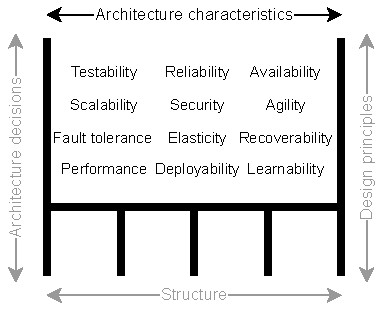
\includegraphics[width=1\textwidth]{img/ArchitectureCharacteristics}}\\ % Pfad
		\source{\cite[Eigene Darstellung in Anlehnung an][17]{Ford2020}} % Quelle
		\label{fig:ArchitectureCharacteristics}
	\end{minipage}
\end{figure}

Einige Merkmale schließen sich gegenseitig aus, wie es beispielsweise bei hoher \textit{Konsistenz}, hoher \textit{Verfügbarkeit} und hoher \textit{Ausfalltoleranz} in einem verteilten System der Fall ist. Die Unmöglichkeit diese drei \textit{Architekturmerkmale} gleichzeitig in einem verteiltem System zu garantieren, wird als \textit{CAP-Theorem} bezeichnet. Die Abkürzung CAP steht für die englischen Architekturmerkmale \textit{Consistency}, \textit{Availability} und \textit{Partition tolerance}.\footnote{\cite[vgl.][]{IBM2019}}

Der dritte Faktor sind die \textit{Architekturentscheidungen}, welche für eine Software relevant sind. Ein Softwarearchitekt gibt Regeln für das System vor, welche eingehalten werden müssen. Beispielsweise wird bei einer Schichtenarchitektur entschieden, dass nur die Business- und Serviceschichten die Datenbankschicht erreichen dürfen. Die Präsentationsschicht hingegen darf dies nicht. Diese Regeln setzen Grenzen für das System und weisen die Entwickler an, wie sie die Anwendung zu realisieren haben.\footnote{\cite[vgl.][17]{Ford2020}} Diese Regeln dürfen, im Gegensatz zu Best Practices, nicht verletzt werden.

Der letzte Aspekt der Softwarearchitektur sind \textit{Designprinzipien}. Diese beinhalten im Gegensatz zu den strikten Regeln, welche bei den Architekturentscheidungen aufgestellt wurden, eher Empfehlungen und Best Practices, welchen gefolgt werden sollte. Ein beispielhaftes Designprinzip wäre es, sofern möglich, immer auf asynchrone Kommunikation zu setzen.\footnote{\cite[vgl.][18\psq]{Ford2020}}

\textbf{Architekturstruktur MVVM}\\
Eine mögliche Architekturstruktur für Webanwendungen ist das \textit{\gls{MVVM}} Entwurfsmuster, welches eine Variante des \textit{\gls{MVC}} Entwurfsmusters darstellt und in vielen Web Frameworks verwendet wird, wie bspw. \textit{Angular}, \textit{Vue.js} oder \textit{React}.

In der nachfolgenden \cref{fig:MVVM} ist das \textit{\gls{MVVM}} Pattern dargestellt, wie es beispielsweise bei Angular eingesetzt wird.

\begin{figure}[hbt!]
	\begin{minipage}[t]{1\textwidth}	
		\caption{MVVM Pattern}
		\frame{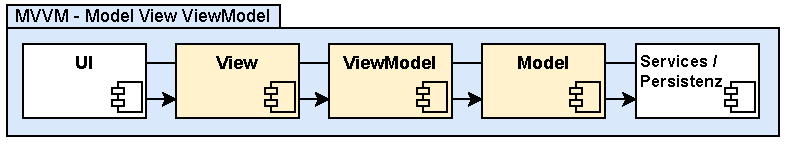
\includegraphics[width=1\textwidth]{img/mvvm}}\\ % Pfad
		\source{\cite[Eigene Darstellung in Anlehnung an][94]{Tremp2021}} % Quelle
		\label{fig:MVVM}
	\end{minipage}
\end{figure}

Das \textit{\gls{MVVM}} Muster besteht aus drei zentralen Komponenten: \textit{Datenmodell (Model)}, \textit{Präsentation (View)} und \textit{Programmsteuerung (ViewModel)}. Das \textit{ViewModel} beinhaltet die Attribute der Geschäftsobjekte, welche von der \textit{View} bei Bedarf konsumiert und angezeigt werden können. Das \textit{Model} beinhaltet die Logik und kann, durch geänderte Daten, Änderungen an der \textit{View} auslösen. Die \textit{View} repräsentiert den Inhalt, der in dem \gls{UI} angezeigt wird. Sie nimmt Nutzerinteraktionen entgegen und steht in bidirektionaler Kommunikation mit dem \textit{ViewModel}, um Werte anzuzeigen oder Input weiter zu reichen.\footnote{\cite[vgl.][95\psq]{Tremp2021}}

\textbf{Designprinzip DDD}\\
Bei dem Designprinzip des \textit{\gls{DDD}} wird eine große Anwendung in kleine, nach Fachlichkeit getrennte, Domänen aufgeteilt. Die Domänen können anhand ihres Nutzens und der Nutzer, welche mit ihr interagieren, identifiziert werden. Eine Domäne ist selbstständig und abgekapselt gegenüber anderen Domänen. Komplexe Fachlichkeiten können in Sub-Domänen einer Domäne abgebildet werden.\footnote{\cite[vgl.][4\psq]{Steyer2020}}

\subsubsection{Angular Frontend}\label{sec:AngularFrontend}

Im Jahr 2009 wurde mit \textit{AngularJS} ein Web Framework für dynamische Webanwendungen veröffentlicht.\footnote{\cite[vgl.][15]{Clow2018}} Angular Versionen sind nach \textit{\gls{SV}} benannt. \textit{AngularJS} bezeichnet das Web Framework Angular in der Major Version 1. Seit der Major Version 2 wird das Web Framework generell als Angular bezeichnet.\footnote{\cite[vgl.][]{Angular2022b}} Zum aktuellen Zeitpunkt (Q1/2022) ist Angular 13, welches im November 2021 erschienen ist, die aktuellste Version.\footnote{\cite[vgl.][]{Thompson2021}}

Durch das Web Framework Angular kann eine \textit{\gls{SPA}} realisiert werden. Bei einer \textit{\gls{SPA}} sind alle Inhalte auf einer einzigen Seite erreichbar, deren Bereiche dynamisch im Browser des Clients nachgeladen werden. Bei Angular wird die Steuerung der angezeigten Inhalte durch den Angular Router vorgenommen. Dieser kann Routen auch nur autorisierten Nutzern ermöglichen und somit Berechtigungslogik abbilden.\footnote{\cite[vgl.][]{Angular2022c}}

Angular Anwendungen sind modular aufgebaut und in Module getrennt. Ein Angular Modul gruppiert Angular Komponenten und Services, welche zu einer Domäne gehören. Angular Module können exportiert werden. Dadurch können Module andere exportierte Module importieren, um deren Funktionen einzubinden.\footnote{\cite[vgl.][]{Angular2022d}}

Eine Angular Komponente stellt eine View dar, welche aus Anzeige, Logik und Styling besteht und damit die drei Technologien verwendet, welche zu Beginn in \cref{sec:Webentwicklung} erläutert wurden.\footnote{\cite[vgl.][]{Angular2022e}} Die Darstellung und Änderung der Inhalte erfolgt über das \gls{MVVM} Pattern. Eine Angular Komponente ist Teil eines Angular Modules und kann von anderen Komponenten in dem Modul referenziert und verwendet werden.

Damit Komponenten untereinander kommunizieren und auf gemeinsam genutzte Daten oder Logik zugreifen können, gibt es Angular Services. Durch Services wird außerdem die Logik, welche zu der View der Komponente gehört, von anderen Operationen getrennt. Dadurch beinhaltet die Komponente nur noch die eigene relevante Logik. Services können durch Konstruktoren Dependency Injection in der Komponente verfügbar gemacht werden und sind anschließend referenzierbar.\footnote{\cite[vgl.][]{Angular2022f}}

Der Code von Angular Applikationen wird durch \textit{webpack} als Modulbundler zu einer \gls{JS} Datei zusammengefasst und anschließend zum Laden an den Client bereitgestellt. Webpack erstellt Pakete, welche die notwendigen \gls{HTML}, \gls{CSS} und \gls{JS} Dateien enthalten. Ebenfalls werden die Referenzen zu eventuellen Assets gesetzt, welche ebenfalls mit veröffentlicht werden. Es werden die Import-Statements jeder Datei gelesen und anhand dieser eingebundenen Dependencies ein zusammenhängendes Bundle von benötigten Bibliotheken erstellt. Die relevante Konfiguration wird in der \texttt{webpack.config.js}-Datei definiert.\footnote{\cite[vgl.][]{Angular2022g}} 

\subsection{Microservices}\label{sec:Microservices}

In diesem Abschnitt werden die Grundlagen zu Microservices erklärt. Microservices sind ein umfangreiches Thema, welches bei ganzheitlicher Betrachtung den Rahmen der Arbeit überschreiten würde. Daher werden nachfolgend nur die Grundlagen erklärt und anschließend Abgrenzungen und Gemeinsamkeiten zu Microfrontends erläutert.

Microservice-Architekturen zählen momentan zu den gefragtesten Technologien in der Softwareentwicklung \footnote{Siehe \cref{fig:StatistikMicroServices} in Anhang \ref{app:Bilder}} und sind nach der Lünendonk Studie 2021 \enquote{Cloud-native Software Development} bei zwei drittel der repräsentativen Unternehmen im Einsatz.\footnote{\cite[vgl.][]{Lünendonk2021}}

Sam Newman definiert Microservices wie folgt: \enquote{Microservices are independently releasable services that are modeled around a business domain.}\footnote{\cite[][18]{Newman2021}}

In der nachfolgenden \cref{fig:MicroservicesFeBe} ist der Unterschied zwischen einer monolithischen Anwendung und einer Microservice-Architektur mit einem monolithischen Frontend dargestellt.

\newpage
\begin{figure}[hbt!]
	\centering
	\begin{minipage}[t]{0.7\textwidth}	
		\caption{Unterschiede monolithische Anwendung zu Microservices}
		\frame{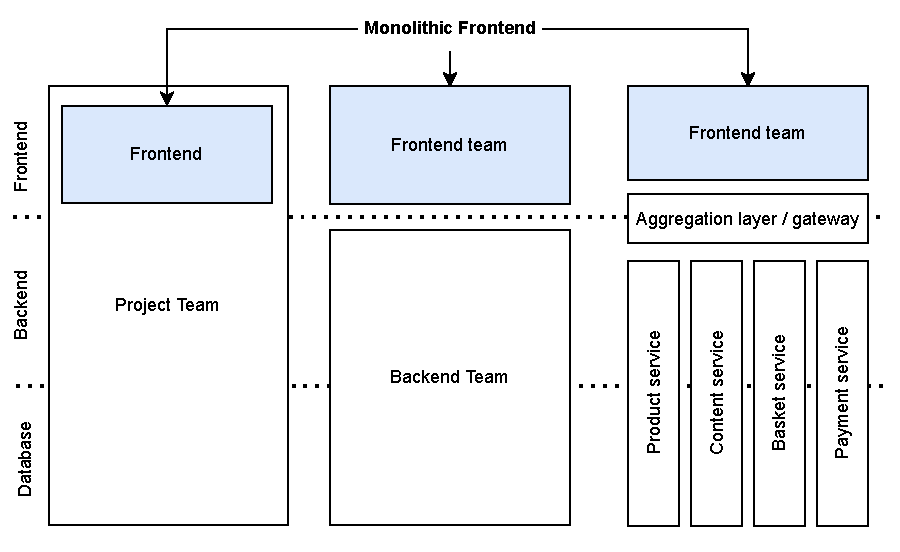
\includegraphics[width=1\textwidth]{img/MicroservicesFeBe}}\\ % Pfad
		\source{\cite[Eigene Darstellung in Anlehnung an][13]{Geers2020}} % Quelle
		\label{fig:MicroservicesFeBe}
	\end{minipage}
\end{figure}

Während die monolithische Anwendung links in der Abbildung das Frontend und das Backend ganzheitlich und ohne Trennungen beinhaltet, kann alternativ das in sich monolithische Frontend von dem monolithischen Backend getrennt sein. Bei einer Microservice-Architektur ist das Frontend ebenfalls vom Backend getrennt, welches wiederum in einzelne funktionale Blöcke aufgeteilt ist, die sogenannten Microservices. Ein Microservice ist durch ein \textit{\gls{API}} aufrufbar und beinhaltet die Logik einer Domäne.

Ein Microservice kann durch die dedizierte Verantwortung einer Domäne unabhängig veröffentlicht, sowie eigenständig getestet und individuell skaliert werden.\footnote{\cite[vgl.][]{Thoenes2015}} Dies ist bei einer monolithischen Anwendung nicht gegeben. Generell können sieben Prinzipien von Microservices herausgestellt werden, durch die sie sich von monolithischen Lösungen abgrenzen.\footnote{\cite[vgl.][16]{Mezzalira2021}} Diese werden nachfolgend erläutert.

\textbf{Modeled Around Business Domains}\\
Nach dem Prinzip des \gls{DDD} ist die Softwarelösung in fachliche Domänen aufgeteilt. Jeder Microservice repräsentiert eine eigene Domäne. Dies hat den Vorteil, dass das System klar strukturiert ist. Das verantwortliche Team der Domäne kennt die Grenzen der eigenen Verantwortung, da diese innerhalb ihrer Domäne liegt. Die Verantwortung anderer Domänen liegt bei anderen Teams.\footnote{\cite[vgl.][16\psq]{Mezzalira2021}}

\textbf{Culture of Automation}\\
Eine hoher Automatisierungsgrad ist bei einer Microservice-Architektur essentiell. Weil die Microservices unabhängig voneinander veröffentlicht werden sollen, empfiehlt es sich alle benötigten Schritte im \textit{\gls{CI/CD}} Prozess zu automatisieren.\footnote{\cite[vgl.][17]{Mezzalira2021}} So kann das Team, welches bspw. für die Werbung verantwortlich ist, seinen Microservice automatisiert neu veröffentlichen. Es muss sich nicht mit den anderen Teams absprechen, solange keine breaking Changes veröffentlicht werden. Es ist nur der eigene Microservice kurzfristig von einem Ausfall während des Veröffentlichungsprozesses betroffen, was für eine starke Unabhängigkeit spricht.

\textbf{Hide Implementation Details}\\
Um Abhängigkeiten zu vermeiden werden alle nicht benötigten Features und Schnittstellen gegenüber anderen Domänen versteckt. Es werden nur benötigte Funktionen über \gls{API}s bereitgestellt. Dadurch behält das Team des Microservices den Überblick, welche Abhängigkeiten zu anderen Domänen bestehen und kann Änderungen bewusst durchführen, ohne bestehende andere Microservices zu beeinflussen.\footnote{\cite[vgl.][17]{Mezzalira2021}}

\textbf{Decentralize Governance}\\
Bei monolithischen Anwendungen werden Architekturentscheidungen ganzheitlich für das gesamte System gefällt, obwohl diese Entscheidung eventuell nicht für jede Domäne optimal ist. Bei Microservices kann jedes Team seine eigenen Entscheidungen fällen. Ob sie beispielsweise synchron oder asynchron kommunizieren und welche Datenbanktechnologie eingesetzt wird, ist jedem Team selber überlassen. Dies sorgt dafür, dass in jeder Domäne die optimale Lösung für den jeweiligen Anwendungsfall zu finden ist. Dennoch müssen übergreifende Entscheidungen und Rahmenbedingungen vorgegeben sowie Standards eingehalten werden.\footnote{\cite[vgl.][17]{Mezzalira2021}}

\textbf{Deploy Independently}\\
Individuelles Deployment ist durch eine hohe Automatisierungsrate zeitsparend realisierbar. Wenn jeder Microservice eine eigene Deploymentpipeline hat, können einzelne Domänen bei Bedarf in einer neueren Version veröffentlicht werden, ohne das andere Domänen beeinträchtigt werden. Bei einer monolithischen Anwendung muss das gesamte System zusammen veröffentlicht werden, was zu einer Ausfallzeit führt und in Summe länger dauert. Microservices können einzeln schneller veröffentlicht werden und bei Bedarf ebenfalls schnell wieder auf einen funktionierenden Stand zurückgerollt werden.\footnote{\cite[vgl.][17]{Mezzalira2021}} 

Das unabhängige Veröffentlichen und ein hoher Automatisierungsgrad im Prozess der Veröffentlichung haben Synergieeffekte, weil der Releaseprozess dadurch pro Durchführung weniger Zeitaufwand benötigt.

\textbf{Isolate Failure}\\
Eine Folge der Auftrennung des monolithischen Backends in einzelne Microservices ist eine erhöhte Ausfallsicherheit. Bei einer monolithischen Anwendung ist das ganze System von einem Ausfall betroffen, bei einer Microservice-Architektur lediglich die Features der betroffenen Domäne. Kunden können weiterhin die Features der anderen Domänen nutzen und bemerken den Ausfall der betroffenen Domäne im besten Fall gar nicht.\footnote{\cite[vgl.][18]{Mezzalira2021}}

\textbf{Highly Observable}\\
Eine der Herausforderungen einer verteilten Microservice-Architektur ist es, den Überblick über alle Domänen zu behalten. Eine monolithische Anwendung als Gesamtsystem ist einfacher zu Überblicken und kann schneller um neue domänenübergreifende Anfragen erweitert werden. Bei einer Microservice-Architektur ist dies mit mehr Aufwand verbunden, welcher aber durch die gewonnene Flexibilität zu rechtfertigen ist.\footnote{\cite[vgl.][18]{Mezzalira2021}} Der höhere Aufwand entsteht durch die Abkapselung der anderen Domänen. Es ist für ein Team einer Domäne nicht direkt ersichtlich, von welchen Features anderer Domänen profitiert werden kann.

Zusammenfassend bringt eine Microservice-Architektur einige Vorteile gegenüber einer monolithischen Architektur. Allerdings ist eine Umstrukturierung der internen Organisation erforderlich, damit Teams unabhängig voneinander sind und Domänentrennung bei Erhaltung des Gesamtüberblickes realisiert werden können.\footnote{\cite[vgl.][18]{Mezzalira2021}}

Die Prinzipien von Microservices lassen sich auf Microfrontends übertragen, was im nachfolgenden \cref{sec:MicrofrontendArchitektur} getan wird.

\subsection{Microfrontend-Architektur}\label{sec:MicrofrontendArchitektur}

In diesem Kapitel werden die Grundlagen von Microfrontends erläutert. Dazu werden zunächst die Gemeinsamkeiten von Microfrontends gegenüber Microservices erläutert sowie Unterschiede abgegrenzt. Anschließend wird das Konzept einer Microfrontend-Architektur präsentiert und Microfrontends aus technischer sowie organisatorischer Sicht vorgestellt.

Microfrontends sind ein möglicher Ansatz der Softwarearchitektur einer Webseite. Anstatt eines monolithischen Frontends ist das Frontend in kleinere, fokussierte Subsysteme aufgeteilt, welche von einem eigenen Team betrieben werden, das sich auch um das dazugehörige Backend kümmert.\footnote{\cite[vgl.][21\psq]{Geers2020}}

In der nachfolgenden \cref{fig:fragments} sind drei Microfrontends dargestellt. Diese werden jeweils von drei verschiedenen Teams betreut und können in unterschiedlichen Web-Frameworks entstanden sein.

\begin{figure}[hbt!]
	\centering
	\begin{minipage}[t]{0.8\textwidth}	
		\caption{Verschiedene voneinander unabhängige Microfrontends}
		\frame{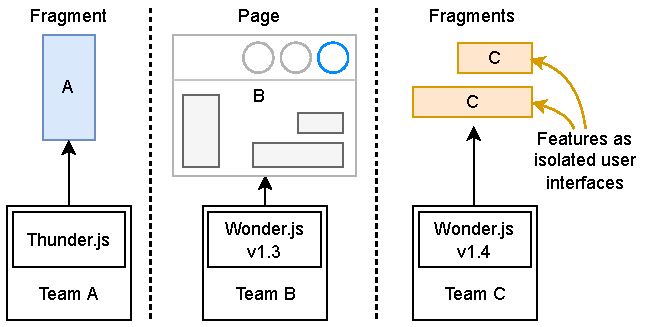
\includegraphics[width=1\textwidth]{img/IsolatedFragments}}\\ % Pfad
		\source{\cite[Eigene Darstellung in Anlehnung an][8]{Geers2020}} % Quelle
		\label{fig:fragments}
	\end{minipage}
\end{figure}

Team A und C steuern jeweils Fragmente bei. Team B ist verantwortlich für die eigentliche Seite, welche die anderen Fragmente später einbindet, und lässt Platzhalter an den Stellen frei, wo die Fragmente in Zukunft platziert werden sollen. Das Zusammenfügen der einzelnen Fragmente auf der Seite erfolgt durch die Konfiguration von Team B und ist nachfolgend in der \cref{fig:frontendintegration} dargestellt.

\newpage 
\begin{figure}[hbt!]
	\centering
	\begin{minipage}[t]{0.8\textwidth}	
		\caption{Frontend Integration der einzelnen Microfrontends}
		\frame{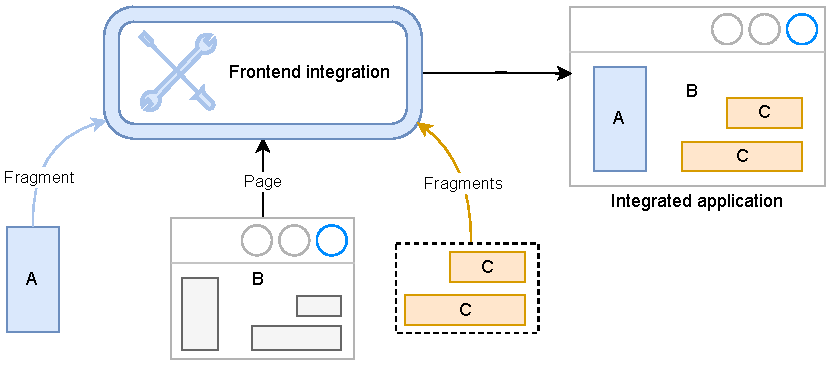
\includegraphics[width=1\textwidth]{img/FrontendIntegration}}\\ % Pfad
		\source{\cite[Eigene Darstellung in Anlehnung an][10]{Geers2020}} % Quelle
		\label{fig:frontendintegration}
	\end{minipage}
\end{figure}

Die Fragmente und die Seite mit den noch leeren Platzhaltern werden durch die sogenannte \textit{Frontend integration} zusammengesetzt und es entsteht eine Web-Anwendung bestehend aus mehreren Microfrontends, was für den Anwender idealerweise nicht ersichtlich ist. Ein Beispiel für eine zusammengesetzte Microfrontend-Applikation ist in der nachfolgenden \cref{fig:TractorStoreMicrofrontend} dargestellt.

\begin{figure}[hbt!]
	\centering
	\begin{minipage}[t]{0.8\textwidth}	
		\caption{Eine aus Microfrontends bestehende Webseite}
		\frame{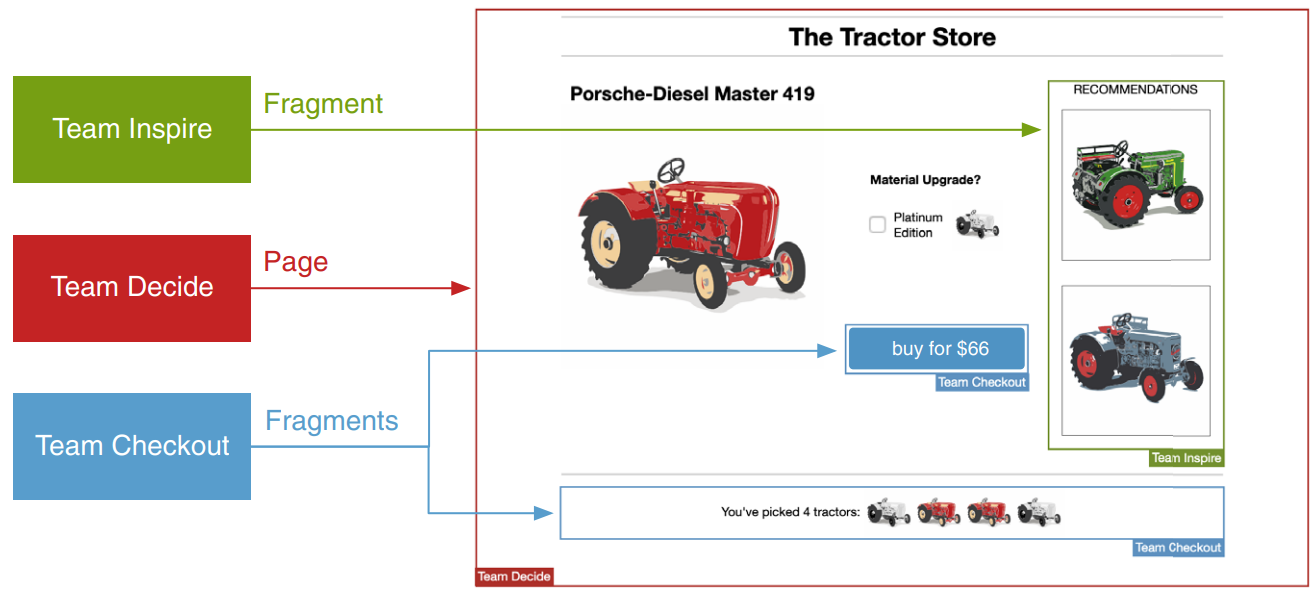
\includegraphics[width=1\textwidth]{img/TractorStoreMicrofrontend}}\\ % Pfad
		\source{\cite[][9]{Geers2020}} % Quelle
		\label{fig:TractorStoreMicrofrontend}
	\end{minipage}
\end{figure}

Das Frontend des beispielhaften Traktorshops ist aus den Fragmenten drei verschiedener Teams zusammengesetzt. \textit{Team Decide} stellt die eigentliche Seite mit den Platzhaltern zur Verfügung, in welche die Fragmente der Teams \textit{Inspire} und \textit{Checkout} eingebunden werden. Für den Shopbenutzer ist diese Trennung in drei Teams nicht ersichtlich und die Webseite erscheint als eine zusammengehörige Komponente.

\subsubsection{Gemeinsamkeiten und Abgrenzungen zu Microservices}\label{sec:AbgrenzungenMicroservices}

Im \cref{sec:Microservices} wurden das Konzept, die Vorteile und Anwendungsfälle von Microservices vorgestellt. In diesem Abschnitt werden weiterführend Abgrenzungen und Gemeinsamkeiten von Microservices gegenüber Microfrontends herausgearbeitet, bevor im nachfolgenden \cref{sec:MicrofrontendArchitekturTechnisch} die Microfrontend-Architektur erklärt wird.

Microfrontends und Microservices unterscheiden sich durch ihren Scope. Microservices sind für das Backend einer Anwendung zuständig und befinden sich hinter der \gls{API}. Microfrontends sind für das Frontend einer Anwendung zuständig und rufen die \gls{API} auf.

Abseits vom Scope gibt es aber viele Gemeinsamkeiten. So lassen sich die Prinzipien von Microservices, welche im vorherigen Abschnitt dargestellt wurden, auf Microfrontends übertragen.\footnote{\cite[vgl.][18-20]{Mezzalira2021}} In Anhang \ref{app:Bilder} in \cref{fig:MonolithicMicrofrontend} ist eine Gegenüberstellung von einem monolithischen Frontend zu einer Applikation mit Microfrontends zu sehen. Bei der Applikation mit Microfrontends ist das Frontend in mehrere unabhängige und nach Fachlichkeit getrennte Teile aufgetrennt, genau wie es bei Microservices im Backend der Fall ist. Dadurch sind vertikale Teams in der Lage die gesamte Verantwortung in ihrer Domäne zu übernehmen. Beispielsweise ist das \textit{Product Team} für den \textit{Product Microservice} sowie für das \textit{Product Microfrontend} zuständig und verwaltet somit die gesamte Produkt-Domäne.

\subsubsection{Microfrontend-Architektur aus technischer Sicht}\label{sec:MicrofrontendArchitekturTechnisch}

\enquote{Microfrontends are not appropriate for every application because of their nature and the potential complexity they add at the technical and organizational levels.}\footnote{\cite[][20]{Mezzalira2021}}

Damit die Vorteile von Microfrontends genutzt werden können, sollten die Anforderungen geprüft und die Architektur dahingehend geplant werden. Eine Microfrontend-Architektur kann nach Mezzalira durch vier Prinzipien beschrieben werden. 

Die vier Prinzipien lauten: \textit{business domain representation}, \textit{autonomous codebase}, \textit{independent deployment} und \textit{single-team ownership}. Ein Microfrontend repräsentiert dementsprechend eine Geschäftsdomäne, welche autonom entwickelt sowie unabhängig veröffentlicht werden kann und von einem eigenen Team betreut wird.\footnote{\cite[vgl.][23]{Mezzalira2021}}

Nachfolgend wird das sogenannte \textit{Microfrontend Descision Framework} vorgestellt. Es beschreibt Kriterien, anhand welcher passende Architekturentscheidungen für die Anwendung getroffen werden können und beinhaltet vier Kernaspekte:\footnote{\cite[vgl.][24]{Mezzalira2021}}

\begin{compactitem}
	\item Einheitliche Definitionen in der eigenen Architektur
	\item Zusammensetzung
	\item Weiterleitung
	\item Kommunikation untereinander
\end{compactitem}

Die einzelnen Aspekte werden nachfolgend im Detail erklärt, weil sie wichtige Grundlagen zum Verständnis von Microfrontend-Architekturen bilden.

\textbf{Einheitliche Definition von Microfrontends in der eigenen Architektur}\\
Zunächst muss ein einheitliches Verständnis von einem Microfrontend gewonnen werden. Dafür wird unterschieden, ob es sich um eine vertikale Trennung in Domänen nach dem \gls{DDD} Konzept, oder um eine horizontale Trennung von mehreren Microfrontends auf der gleichen Seite, wie in der nachfolgenden \cref{fig:HorizontalVerticalSplit} dargestellt, handelt.

\begin{figure}[hbt!]
	\begin{minipage}[t]{1\textwidth}	
		\caption{Horizontale und vertikale Trennung von Microfrontends}
		\frame{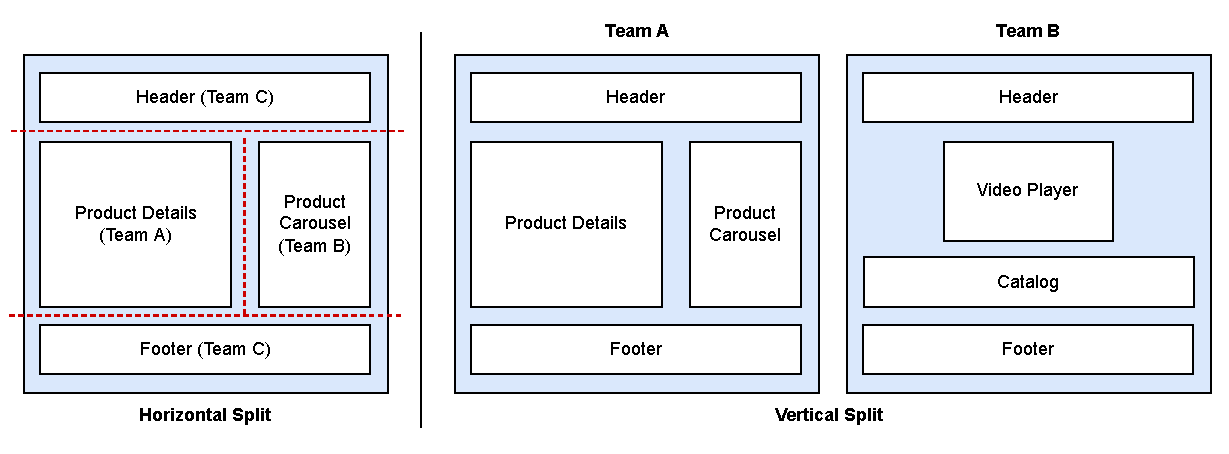
\includegraphics[width=1\textwidth]{img/HorizontalVerticalSplit}}\\ % Pfad
		\source{\cite[Eigene Darstellung in Anlehnung an][24]{Mezzalira2021}} % Quelle
		\label{fig:HorizontalVerticalSplit}
	\end{minipage}
\end{figure}

Bei dem \gls{DDD} geht es darum, die Anwendung in Fachdomänen aufzutrennen. Eine Domäne kann wiederum in mehrere Subdomänen aufgeteilt werden, welche sich in drei Typen unterscheiden lassen:\\
In \textit{funktionale Subdomänen}, welche den Hauptnutzen der Domäne repräsentieren. \\
In \textit{unterstützende Subdomänen}, welche zwar die funktionale Subdomäne unterstützen, aber keinen direkten Wert beisteuern.\\
In \textit{generische Subdomänen}, welche der übergreifenden Plattform dienen und den Prozess abrunden. Sie haben keinen direkten Bezug zur Domäne, sind aber für die Erfüllung des übergreifenden Nutzens relevant (bspw. die Authentifizierung auf einer Webseite).\footnote{\cite[vgl.][24\psqq]{Mezzalira2021}} 

Im Falle der in \cref{fig:HorizontalVerticalSplit} dargestellten vertikalen Trennung wird in die Domänen \textit{Video} und \textit{Produkt} unterschieden, welche jeweils von einem Team betreut werden. Die Teams mit ihren Domänen sind voneinander unabhängig und abgekapselt. Sollten Zugriffe domänenübergreifend notwendig sein, werden diese über ein \gls{API} realisiert.

\textbf{Zusammensetzung von Microfrontends}\\
Ebenfalls muss vorab entschieden werden, wann die Microfrontends zusammengesetzt werden (engl. \textit{composition}). Dies kann an drei verschiedenen Stellen geschehen:\footnote{\cite[][29]{Mezzalira2021}}
\begin{compactitem}
	\item \textit{Client-side Composition}
	\item \textit{Edge-side Composition}
	\item \textit{Server-side Composition}
\end{compactitem}

Bei der \textit{Client-side Composition} werden die einzelnen Microfrontends vom Client einzeln aus einem \gls{CDN}, oder falls dort nicht vorhanden, direkt aus der Quelle geladen und am Client im Browser zusammengesetzt.

Bei der \textit{Edge-side Composition} wird das Zusammensetzen der einzelnen Microfrontends im \gls{CDN} vollzogen und die Anwendung als Ganzes an den Client ausgeliefert.

Die \textit{Server-side Composition} hingegen setzt die Microfrontends bereits auf einem Server zusammen und gibt sie als Ganzes an das \gls{CDN} weiter, welches die Seite zwischenspeichert und anschließend an den Client ausliefert.

\textit{Client-side} und \textit{Server-side Composition} werden in den \crefrange{sec:ServerSideComposition}{sec:ClientSideComposition} ausführlicher behandelt. Auf eine detailliertere Erklärung von \textit{Edge-side Composition} wird verzichtet, da es dem Konzept der\textit{ Server-side Composition} ähnelt und für den weiteren Verlauf der \dokumententyp{} keine Relevanz hat.

\textbf{Weiterleitung von Microfrontends}\\
Nachdem der Ort der Zusammenstellung der Microfrontends bestimmt wurde, muss eine Technik gewählt werden, um zwischen den Ansichten verschiedener Microfrontends zu wechseln. Bezogen auf den vorherigen Punkt \textit{Zusammensetzung} muss entschieden werden, ob das Weiterleiten (engl. \textit{Routing}) auf dem Server, dem \gls{CDN} oder am Client passiert.

Wenn die Anwendung auf dem Server zusammengesetzt wird, muss sie auch dort gerouted werden, weil sich die Logik sowie die anderen Ansichten serverseitig befinden. Die gerouteten Ansichten können dann vom \gls{CDN} zwischengespeichert werden, wenn sich die Ansichten nicht individuell pro Mandant oder User unterscheiden.\footnote{\cite[vgl.][31]{Mezzalira2021}}

Bei dem Einsatz von \textit{Edge-side Composition} wird das Routing über \gls{URL} realisiert und die Microfrontends werden vom \gls{CDN} Server zusammengesetzt.\footnote{\cite[vgl.][32]{Mezzalira2021}} Es besteht in diesem Fall nicht viel Entscheidungsfreiraum beim Routing, was einer der Gründe ist, warum \textit{Edge-side Composition} im Rahmen der Thesis nicht weiter verfolgt wird.

Das Routing am Client durchzuführen bringt die meiste Flexibilität, da die einzelnen Microfrontends nach Bedarf und individueller Konfiguration des Clients geladen und zwischengespeichert werden können.

Die Art des clientseitigen Routings ist in \gls{SPA}s wiederzufinden, welche bereits vorher in \cref{sec:AngularFrontend} beschrieben wurden. Eine \gls{SPA} kann als \textit{Application Shell} fungieren, indem sie abhängig des aktuellen Router- und Nutzerstatus andere Microfrontends einbindet und anzeigt. Die \textit{Application Shell}s bieten Querschnittsaspekte, wie bspw. Routing, Authentifizierung und Autorisierung, von welchen die Microfrontends profitieren können und über die ein komplexes, individuelles Routing abgebildet werden kann. Die Konzepte der \textit{Application Shell} und der eingebundenen Microfrontends werden im nachfolgenden \cref{sec:Portalapplikationen} ausführlich behandelt.

Das clientseitige Routing kann auch ohne eine \gls{SPA} lediglich über \gls{URL}s realisiert werden, zwischen welchen der Benutzer navigieren kann.\footnote{\cite[vgl.][32]{Mezzalira2021}} Dabei springt der Benutzer aber von Seite zu Seite, verliert eventuell gespeicherte Informationen und wird mit Ladezeiten je Seite konfrontiert.

\textbf{Kommunikation von Microfrontends untereinander}\\
Optimalerweise laufen Microfrontends vollkommen autark und haben nach dem \gls{DDD} Prinzip keine Überschneidungen zu anderen Domänen. Dies ist bei größeren Applikationen aber nicht gegeben, weil beispielsweise Microfrontends auf die Nutzerdomäne zugreifen müssen, um Informationen über den aktuellen Benutzer erhalten zu können.

Besonders bei mehreren Microfrontends auf der gleichen Seite ist das Verwalten einer konsistenten und kohärenten \gls{UX} herausfordernd. Zusätzlich erschwert die Domänenverwaltung durch verschiedene Teams das Kommunizieren von Microfrontends untereinander.\footnote{\cite[vgl.][33]{Mezzalira2021}}

Die Kommunikation kann, bei horizontaler Trennung, über vier verschiedene Arten erfolgen: \textit{Event emitter}, \textit{Custom events}, \textit{Web Storage} oder \textit{Query Strings}. Bei vertikaler Trennung sind ist die Kommunikation nur über einen \textit{Web Storage} und \textit{Query Strings} möglich.

Sind die Microfrontends auf der gleichen Seite eingebunden, kann über Events kommuniziert werden. Eine zentrale Stelle (bspw. die \textit{Application Shell}) versendet Events und Microfrontends können auf diese Eventbenachrichtigungen reagieren. Dies ist über das \textit{CustomEvent} Interface von Javascript möglich.\footnote{\cite[vgl.][]{MDNWebDocs2022b}}

Die Daten können ebenfalls über \textit{Event Emitter} geteilt werden, wie in \cref{fig:MFSharingDataEventEmitter} in Anhang \ref{app:Bilder} dargestellt. Dafür muss ein \gls{Eventbus} in jedes Microfrontend eingefügt werden, auf welchem Nachrichten versendet werden können.\footnote{\cite[vgl.][33]{Mezzalira2021}}

Eine weitere Möglichkeit zum Datenaustausch ist das Teilen von Informationen über einen gemeinsamen \textit{Web Storage} (siehe \cref{fig:MFSharingDataWebStorage} in Anhang \ref{app:Bilder}). Es wird ein \textit{Web Storage} verwendet, welcher von Microfrontends der gleichen Subdomain erreicht werden kann. Dort liegen Informationen des Benutzers, auf welche das Microfrontend zurückgreifen kann.\footnote{\cite[vgl.][34]{Mezzalira2021}}

\textbf{Zusammenfassung Microfrontend Decision Frameworkes}\\
In der nachfolgenden \cref{tab:ZusammenfassunfMFFramework} ist eine Zusammenfassung des Microfrontend Decision Frameworkes dargestellt.

\begin{table}[hbt]
	\centering
	\begin{minipage}[t]{1\textwidth} % Breite, z.B. 1\textwidth		
		\caption{Zusammenfassung des Microfrontend Decision Framework} % Überschrift
		\begin{tabular}{|
				l|ccc|}
			\midrule
			\textbf{Microfrontend definition\quad\quad\quad}&\textbf{Composition}&\textbf{Routing}&\textbf{Communication}\\
			\midrule
			\multirow{4}{*}{Horizontal}
			&Client side 	&Client side	&Event emitter\\ 
			&Server side 	&Server side	&Custom events\\
			&Edge side 		&Edge side		&Web storage\\
			&				&				&Query strings\\						
			\midrule
			\multirow{3}{*}{Vertical}
			&Client side	&Client side	&Web Storage\\ 
			&Server side	&Server side	&Query Strings\\
			& 				&Edge side		&\\
			\midrule
		\end{tabular}
		\newline
		\source{\cite[Eigene Darstellung in Anlehnung an][35]{Mezzalira2021}}
		\label{tab:ZusammenfassunfMFFramework}
	\end{minipage}
\end{table}

Die Tabelle zeigt, dass nicht alle Ausprägungen einer Kategorie miteinander kombinierbar sind. Die erste Entscheidung muss bezüglich der Definition getroffen werden. Eine vertikale Definition hat zur Folge, dass beim Routing und bei der Kommunikation weniger Optionen verfügbar sind.

Die Vorteile und Nachteile lassen sich aus den eingangs erklärten Prinzipen von Microfrontends ableiten und werden zur Übersicht nachfolgend noch einmal erklärt.

\textbf{Vorteile gegenüber einem monolithischen Frontend}\\
Der primäre Vorteil einer Microfrontend-Architektur ist die gewonnene Flexibilität. Jedes Team ist selbstverantwortlich für ihr zugewiesenes Microfrontend. Sie sind in der Lage selbstständig Architekturentscheidungen zu treffen, welche zu ihren Aufgaben und Problemen passen. Ebenfalls können bei Bedarf neue Softwarestände durch die eigenen Pipelines veröffentlicht werden, ohne andere Microfrontends zu beeinflussen. 

Des Weiteren wird das Microfrontend nicht durch andere Ausfälle beeinflusst. Hat beispielsweise das für die Werbung einer Seite verantwortliche Team eine Störung, kann das Team verantwortlich für die Kaufabwicklung ohne Auswirkungen weiter agieren.\footnote{\cite[vgl.][19\psq]{Mezzalira2021}} So ist das nicht direkt betroffene Team weiterhin nicht abhängig und der Benutzer bemerkt die Störung außerhalb der betroffenen Domäne ebenfalls nicht.

Darüber hinaus ist durch die Trennung nach Domänen in eigenverantwortliche Teams eine klare Strukturierung der Verantwortung gegeben, welche bei der Organisation der Gesamtwebseite von Vorteil ist. Auch ist eine verbesserte Skalierbarkeit gegeben, sodass modulare Microfrontends mehrfach nach Bedarf eingebunden werden können (\textit{\gls{DRY}} Prinzip).

\textbf{Nachteile gegenüber einem monolithischen Frontend}\\
Nachteile einer Microfrontend-Architektur gegenüber einem monolithischen Ansatz sind in den Aspekten Redundanz, Konsistenz und Heterogenität zu finden.\footnote{\cite[vgl.][17]{Geers2020}}

\textbf{Redundanz}\\
In Microfrontend-Architekturen sind Redundanzen nicht zu vermeiden. So hat jedes Team ein eigenes Repository, eine eigene Deployment-Pipeline und einen eigenen Ort zum Hosten des Microfrontends.\footnote{\cite[vgl.][17\psq]{Geers2020}} Ein eigenes Repository ist zwar hilfreich, um sich als Team selbstständiger zu organisieren, aber es besteht auch die Möglichkeit ein Monorepo übergreifend zu verwenden. Dort sind alle Microfrontends der Applikation gleichzeitig enthalten. Alle Microfrontends können auf geteilte Bibliotheken in dem Monorepo zugreifen. Dies erfordert eine gute Zusammenarbeit der einzelnen Teams und eine strikte Organisation des Repositories, was mit Mehraufwand einhergeht.\footnote{\cite[vgl.][153\psq]{Mezzalira2021}}

Durch den Aspekt, dass das vorher monolithische Frontend in kleinere Fragmente aufgeteilt wurde, welche alle selbstständig lauffähig sind, kommt es zu mehrfach geladenem Code.\footnote{\cite[vgl.][19]{Geers2020}} Beispielsweise muss das Web Frontend Framework Angular für jedes Microfrontend geladen werden oder es müssen mehrere verschiedene Web Frontend Frameworks geladen werden. Bei einer monolithischen Anwendung dahingegen wird nur ein Web Frontend Framework benötigt.

\textbf{Konsistenz}\\
Der Microfrontend Ansatz verlangt, wie in \cref{fig:MicroFrontendBigPicture} zu sehen, die Aufteilung in eigenständige, vertikal agierende Teams. Diese Teams sollen nach Möglichkeit alles selbstständig betreiben, vom Frontend über das Backend bis hin zur Datenbank. Nun kann es vorkommen, dass ein Team Daten von einem anderen Team benötigt. Ein direkter Zugriff oder eine geteilte Datenbank würde die Domänentrennung verletzen. 

Aus diesem Grund muss das Team, welches Daten eines anderen Teams benötigt, die Daten replizieren. Das Replizieren von Datenbeständen ist notwendig, damit aus Gründen der Unabhängigkeit und Ausfallsicherheit auf direkte Zugriffe verzichtet werden kann.
Die Replizierung der Daten hat den Nachteil, dass Abhängig von den Replizierungsintervallen unter Umständen veraltete Datenbestände verwendet werden. Darüber hinaus werden doppelte Ressourcen (Speicher- und Rechenkapazität) benötigt.\footnote{\cite[vgl.][18]{Geers2020}} 

Auf eine Replizierung kann verzichtet werden, wenn die Schnittstellen von Domänen in begründeten Fällen doch zur Verfügung gestellt werden. Dies könnte beispielsweise bei weniger relevanten Daten der Fall sein, bei denen ein temporärer Ausfall die Kernfunktion nicht beeinträchtigt.

\textbf{Heterogenität}\\
Da die Teams unabhängig voneinander sind, steht es ihnen frei, welche Technologie sie verwenden. So können alle Microfrontends einer Applikation einheitlich in Angular 12 geschrieben sein. Es besteht aber auch die Möglichkeit verschiedene Versionen der gleichen Technologie zu verwenden. Ein Angular 11 Microfrontend kann in eine Angular 12 Application Shell eingebunden werden. 
Es können aber auch andere Web Frontend Frameworks verwendet werden, also an Stelle von Angular beispielsweise Vue.js oder React. Allerdings erschweren heterogene Technologien den Informationsaustausch der Teams untereinander und einzelne Entwickler können nicht so einfach ohne Weiterbildung zwischen den Teams wechseln. 

Einheitliches Design ist ein wichtiger Aspekt einer funktionierenden Software. Es gibt dem User das Gefühl sich durchgehend auf einer Webseite aufzuhalten. Durch ein \textit{Design System}, eine verbindliche Vorgabe zur Einhaltung eines stringenten Designs für alle beteiligten Teams der Applikation, kann eine einheitliche Webseite erschaffen werden. Auch wenn diese im Hintergrund aus vielen autonomen Microfrontends besteht. Durch die einheitlichen Vorgaben und das stringente Design wird dem Benutzer ein stimmiges \gls{UI}/\gls{UX} Erlebnis ermöglicht.\footnote{\cite[vgl.][214\psqq]{Geers2020}}

Ein \textit{Design System} kann durch einen \textit{Style Guide} realisiert werden, welcher Styles in Form von Schriftarten, Farben und Grafiken vorgibt. Alternativ kann eine \textit{Komponentenbibliothek} zur Verfügung gestellt werden, welche Elemente zum Einbinden in Microfrontends in Form von Formularelementen, Navigationselementen oder Anzeigeelementen liefert.\footnote{\cite[vgl.][215]{Geers2020}} Ein \textit{Design System} zu implementieren und zu Pflegen bedeutet jedoch Mehraufwand, welcher in Kauf genommen werden muss.

Zusammenfassend kann also gesagt werden, dass bei einer Microfrontend-Architektur die Vorteile Flexibilität, Unabhängigkeit und Übersicht nur durch Mehraufwand in der Organisation sowie Redundanz realisierbar sind. Die Nachteile sind durch Mehraufwand kompensierbar, was bei vorheriger Planung und Überprüfung der Architektur gut zu bewältigen ist.

\textbf{Wirkungsbereiche von Microfrontend-Architekturen}\\    
Microfrontend-Architekturen besitzen Vor- und Nachteile. Diese besondere Form der Softwarearchitektur ist nicht für alle Arten von Softwarelösungen geeignet. Wo diese Architekturen empfehlenswert sind und wo sie nicht gerechtfertigt sind, wird nachfolgend erläutert.

Eine Microfrontend-Architektur bietet sich für große, verteilte Softwarelösungen an. Der Bedarf nach Flexibilität und Skalierbarkeit tritt erst ab einem gewissen Umfang der Softwarelösung auf. Bei kleineren Projekten sind Kosten und Schnelligkeit entscheidender.\footnote{\cite[vgl.][19]{Geers2020}}

Die angezeigten Frontends dynamisch auszutauschen funktioniert am besten clientseitig durch \gls{SPA}s. Serverseitiges Rendering erfordert ein erneutes Laden des Inhaltes, was zwar technisch keine Herausforderung darstellt, jedoch nicht so flüssig und unbemerkt wie clientseitige Komposition abläuft. Smartphone Apps als Microfrontend zu realisieren ist schwieriger, da die Betreiber von App Stores strikte Kontrollen des Inhaltes durchführen, bei denen jedes Microfrontend in jeder Version überprüft werden müsste. Dadurch schwinden die flexiblen, unabhängigen Vorteile von Microfrontends.\footnote{\cite[vgl.][19\psq]{Geers2020}}

Eine monolithische Anwendung in viele einzelne Teile aufzutrennen bringt Vorteile und Nachteile mit sich, welche im vorherigen Abschnitt erläutert wurden. Es muss vermehrter organisatorischer Aufwand in Kauf genommen werden. Dieser entsteht durch zusätzliche Abstimmung der Teams untereinander, bspw. für einheitliche Namespaces und Trennung der Verantwortung. Die Aufteilung einer monolithischen Anwendung in ein verteiltes System sorgt für zusätzliche Komplexität. Den verantwortlichen Teams muss die gewonnene Flexibilität wichtiger sein, als der Aufwand und die Komplexität.\footnote{\cite[vgl.][20]{Geers2020}}

\enquote{Microfrontends are a sensible option when we are working on software that requires an iterative approach and long-term maintenance, when we have projects that require multiple teams to work on the same application, or when we want to replace a legacy project in an iterative way.}\footnote{\cite[][21]{Mezzalira2021}}

Eine Microfrontend-Architektur ist nicht effektiv, wenn nur wenige Entwickler an der Softwarelösung arbeiten. Außerdem müssen die Domänen und Verantwortlichkeiten der Teams gut gegeneinander abgetrennt sein, weil es ansonsten zu Unsicherheiten und Verständnisproblemen der Teams untereinander kommen kann.\footnote{\cite[vgl.][21]{Geers2020}}

\subsubsection{Microfrontend-Architektur aus organisatorischer Sicht}\label{sec:MicrofrontendArchitekturOrganisatorisch}

Eine Microfrontend-Architektur hat neben den technischen Aspekten auch organisatorische Unterschiede zu herkömmlichen Architekturen. Einige dieser Aspekte, wie vertikale Teams, notwendige Abstimmungen und geteiltes Wissen wurden bereits in den vorherigen Abschnitten beiläufig erwähnt und werden nachfolgend noch einmal strukturiert erklärt.

\textbf{Organisation der Teams}\\
Es existieren verschiedene Möglichkeiten die Teams bei einer Microfrontend-Architektur zu organisieren. In der nachfolgenden \cref{fig:TeamDepth} wird zwischen ausschließlich im Frontend agierenden Teams, Full-Stack Teams und vollständig autonomen Teams unterschieden.

\begin{figure}[hbt!]
	\centering
	\begin{minipage}[t]{0.85\textwidth}	
		\caption{Organisationsmöglichkeiten der Microfrontend Teams}
		\frame{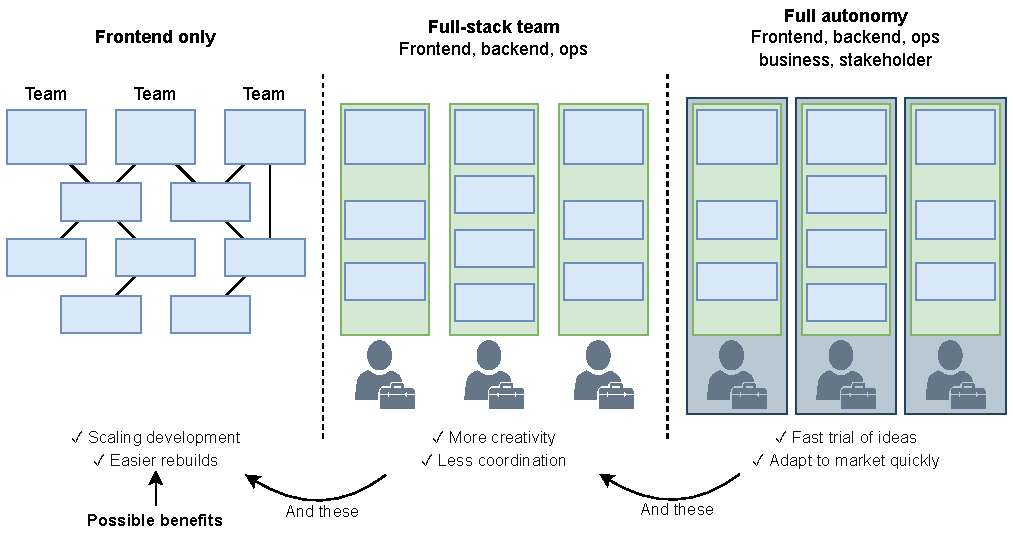
\includegraphics[width=1\textwidth]{img/TeamDepth}}\\
		\source{\cite[Eigene Darstellung in Anlehnung an][240]{Geers2020}} % Quelle
		\label{fig:TeamDepth}
	\end{minipage}
\end{figure}

Beim monolithischen Ansatz ist ein großes Team für die ganze Anwendung verantwortlich. Bei \textit{Frontend only} Teams sind es mehrere, kleine Teams, die jeweils einen bestimmten Bereich des Frontends betreuen. Dies hat den Vorteil, dass die Entwickler in den kleinen Teams sich besser mit den Fachlichkeiten auskennen.\footnote{\cite[vgl.][241]{Geers2020}}

Ebenfalls besteht die Möglichkeit die Teams vertikal aufzuteilen, wodurch jedes Team die Full-Stack Verantwortung für seinen Teilbereich hat. Dies hat den Vorteil, dass weniger Abstimmung notwendig ist, da Frontend und Backend der gleichen Domäne mitsamt der dazwischen liegenden Schnittstellen bei den selben Entwicklern liegen. Ebenfalls werden Full-Stack Teams aus Personen mit diversen fachlichen Wissensständen zusammengesetzt, was die Kreativität der Problemlösung und Qualität des Ergebnisses fördern kann.\footnote{\cite[vgl.][241]{Geers2020}}

Werden die Stakeholder auch noch in das Full-Stack-Team integriert, so kann von einem vollständig autonomen Team gesprochen werden. Wenn die Stakeholder, wie bspw. Marketing, Kunden oder Support, direkt in den Problemlösungsprozess integriert werden, kann von noch kreativeren Blickwinkeln profitiert und die \gls{TTM} noch weiter reduziert werden.\footnote{\cite[vgl.][242]{Geers2020}}

\textbf{Wissensverteilung}\\
Das Wissen übergreifend über autonome Teams hinweg zu verteilen geschieht nicht automatisch, ist aber dennoch ein wichtiger Prozess. Die Mitglieder von vertikalen Teams treffen sich in sogenannten \gls{COP}, welche horizontal organisierten Expertenkreisen entsprechen. So können Best Practises und Erfahrungen der Teams in den notwendigen technischen Tiefen der jeweiligen Spezialisierungen ausgetauscht werden. In Anhang \ref{app:Bilder} in \cref{fig:VertikaleTeamsWissensaustausch} sind drei autonome Teams dargestellt, welche sich regelmäßig in Expertenkreisen treffen und austauschen. So gibt es beispielsweise einen Expertenkreis für das Themengebiet Frontend, einen für die Datenanalyse und einen für Kubernetes als Infrastrukturplattform.

Das Konzept der \gls{COP}s besteht schon länger, als die Microfrontend-Architektur. Doch es ist bei dieser Art der Teamorganisation besonders wichtig, da der sonst bestehende natürliche Austausch innerhalb eines horizontalen Teams verloren geht. In den \gls{COP}s sollte sich auch auf Standards und Konventionen für Schnittstellen und Namespaces innerhalb eines Projektes geeignet werden.

\textbf{Verwaltung des Codes}\\
Bei klassisch monolithischen Anwendungen gibt es ein Repository für die ganze Applikation. Bei Microservices und -frontends kann es für jede Einheit ein eigenes Repository geben. Dies wird als \textit{Polyrepo} bezeichnet. Alternativ kann aber auch für das ganze Projekt nur ein Repository genutzt werden, welches dann einem \textit{Monorepo} entspricht.

Vorteile eines \textit{Monorepos} sind, dass dadurch die Absprache der Teams untereinander vereinfacht wird, weil der Code des anderen Teams direkt zugänglich ist und eingebunden werden kann. Ebenfalls kann der Code einfacher einheitlich überarbeitet werden, da alle Dateien nebeneinander verfügbar sind.\footnote{\cite[vgl.][152\psqq]{Mezzalira2021}}

\textit{Polyrepos} haben den Vorteil, dass die Autonomie gestärkt wird. Jedes Microfrontend hat sein eigenes Repository und eigene \gls{CI/CD} Pipelines angebunden. Ebenfalls können individuelle Branchingstrategien pro Team verwendet und versehentliche Abhängigkeiten vermieden werden, da Zugriffe zwischen Teams nur über definierte \gls{API}s möglich sind.\footnote{\cite[vgl.][156\psqq]{Mezzalira2021}}

Das Konzept des \textit{Monorepos} wird im Microfrontend-Umfeld kontrovers diskutiert. Einige Autoren sehen Vorteile durch Wiederverwendbarkeit und vereinfachte Abhängigkeiten.\footnote{\cite[vgl.][152\psqq]{Mezzalira2021}} Andere Autoren sehen es jedoch als Antipattern, da Code geteilt wird und somit Autonomie verloren geht.\footnote{\cite[vgl.][258]{Geers2020}}

\textbf{Zusammenfassender Überblick}\\
In der nachfolgenden \cref{fig:MicroFrontendBigPicture} wird ein Gesamtüberblick über die Team-Organisation einer Microfrontend-Architektur gegeben.

\begin{figure}[hbt!]
	\centering
	\begin{minipage}[t]{0.75\textwidth}	
		\caption{Zusammenfassende Darstellung Microfrontends}
		\frame{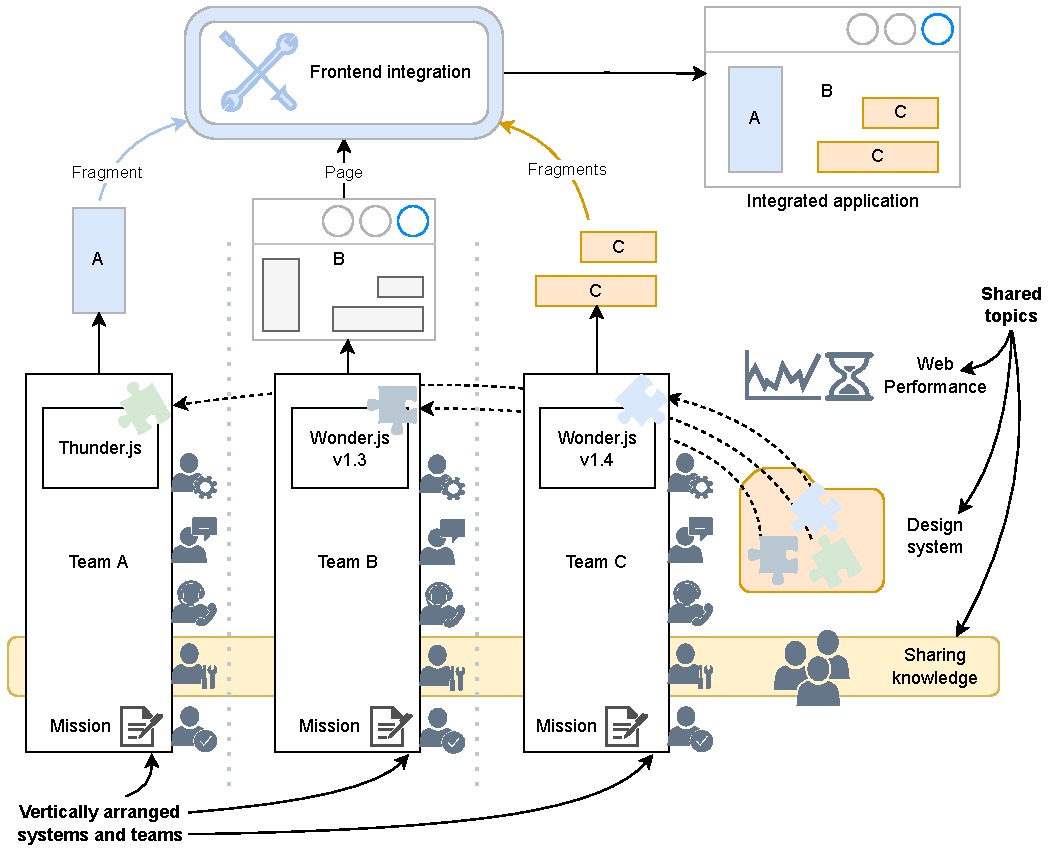
\includegraphics[width=1\textwidth]{img/MicroFrontendBigPicture}}\\
		\source{\cite[Eigene Darstellung in Anlehnung an][5]{Geers2020}} % Quelle
		\label{fig:MicroFrontendBigPicture}
	\end{minipage}
\end{figure}

Es ist zu sehen, wie die einzelnen Microfrontends verschiedener, vertikal organisierter Teams zu einer zusammenhängenden Lösung zusammengefügt werden. Die vertikale Trennung nach Domänen, realisiert mit einem Team pro Domäne, ergänzt sich mit dem horizontalen Teilen von Wissen, Design- und Architekturentscheidungen. Auch können verschiedene Technologien je Team eingesetzt werden, was die Teams unabhängiger voneinander agieren lässt. Die Stakeholder der Domäne sind ebenfalls mit in den Entwicklungsprozess integriert, was das direkte Erstellen von Lösungen, passend zu den Anforderungen, ermöglicht.

\subsection{Portalapplikationen}\label{sec:Portalapplikationen}

In diesem Kapitel wird das Konzept von Portalapplikationen erklärt. Portalapplikationen können in verschiedenen Formen realisiert werden. Im einfachsten Fall durch Hyperlinks, welche im nachfolgenden \cref{sec:PortalapplikationenHyperlinks} vorgestellt werden. Ebenfalls ist die Realisierung einer Portalshell mit Querschnittsfunktionen möglich, welche im darauffolgenden Abschnitt erläutert wird.

Eine Portalapplikation stellt die übergeordnete Webseite dar, welche die einzelnen Microfrontends miteinander verbindet.\footnote{\cite[vgl.][121]{Geers2020}} Dies kann auf unterschiedliche Arten realisiert werden, von denen zwei nachfolgend erläutert werden.

\subsubsection{Portalapplikationen durch Hyperlinks}\label{sec:PortalapplikationenHyperlinks}

Portalapplikationen können bereits durch Verlinkungen realisiert werden. In der nachfolgenden \cref{fig:LinksMicroFrontends} ist dies am Beispiel von Google Maps dargestellt. Die Seite \textit{\url{https://www.google.de/maps}} bindet diverse andere Seiten des Alphabet Konzerns ein und macht diese durch Verlinkungen erreichbar.

\begin{figure}[hbt!]
	\centering
	\begin{minipage}[t]{0.5\textwidth}	
		\caption{Verlinkung anderer Webseiten}
		\frame{
\includegraphics[width=1\textwidth]{img/MFLinks}}\\ % Pfad
		\source{Screenshot von Google Maps} % Quelle
		\label{fig:LinksMicroFrontends}
	\end{minipage}
\end{figure}

Hinter jedem der im rechten Bereich der \cref{fig:LinksMicroFrontends} zu sehenden Icons ist eine weitere Seite durch Klicken zu erreichen. So führt der Klick auf das YouTube Icon den Nutzer zu \textit{\url{https://www.youtube.com/}}. Die bisherige Seite \textit{\url{https://www.google.de/maps}} wird verlassen und der Seiteninhalt von YouTube wird dargestellt.

Der Vorteil bei dieser Art der Realisierung einer Portalapplikation besteht darin, dass Verlinkungen sehr einfach und ohne aufwändige Anpassungen einzurichten sind.

Allerdings verliert der Benutzer beim Wechseln der Webseiten seinen Fortschritt oder seine Eingaben. Ebenfalls muss Aufwand seitens der Webseitenbetreiber investiert werden, damit die verlinkten Webseiten einheitlich aussehen, um die Zusammengehörigkeit sowie das Benutzergefühl zu erhalten.\footnote{\cite[vgl.][36]{Steyer2020}}

Durch Hyperlinks kann die Produktpalette eines Unternehmens einheitlich erreichbar gemacht werden. Es können auch Informationen zu einem bestimmten Thema gesammelt werden, wie es beispielsweise bei \url{https://zeef.com/} der Fall ist. Eine Zeef-Seite zum Thema \textit{Microfrontends} ist unter folgendem Link zu finden: \href{https://micro-frontends.zeef.com/elisabeth.engel?ref=elisabeth.engel&share=ee53d51a914b4951ae5c94ece97642fc}{\nolinkurl{micro-frontends.zeef.com}}.\footnote{\cite[vgl.][]{Engel2021}}

\subsubsection{Portalshell}\label{sec:PortalapplikationenPortalshell}

Wenn das Wechseln zwischen verschiedenen Frontends nicht sichtbar geschehen soll, so muss eine Portalshell (engl. \textit{Application Shell}) gewählt werden. Eine Portalshell ist eine Portalapplikation, welche andere Microfrontends nach horizontaler Trennung einbindet. In Anhang \ref{app:Bilder} in \cref{fig:AufgabenShell} ist eine beispielhafte Portalshell dargestellt, welche das clientseitige Routing zwischen verschiedenen Microfrontends übernimmt.

Die Portalshell hat mehrere Aufgaben, welche in der nachfolgenden Liste dargestellt sind:\footnote{\cite[vgl.][45\psq]{Mezzalira2021}}

\begin{compactitem}
	\item Dynamisch Microfrontend Routen laden
	\item \textit{User state} verwalten	
	\item Fehlerbehandlung beim Laden von Microfrontends
	\item Einheitliches Logging ermöglichen
\end{compactitem}

Die Portalshell muss in der Lage sein, die Microfrontends dynamisch zu laden, damit beim Hinzufügen neuer Microfrontends keine neue Veröffentlichung der Portalshell erforderlich ist. Die Links zu den konfigurierten Microfrontends können hierfür bspw. in einer Datenbank abgelegt werden, auf welche die Portalshell zugreifen kann.\footnote{\cite[vgl.][46]{Mezzalira2021}}

Ebenfalls muss die Portalshell den \textit{User state} kennen und bei Bedarf eine Authentifizierung durchführen. Die Portalshell muss verhindern, dass ein \textit{\gls{Deeplink}} aufgerufen werden kann, wenn keine Authentifizierung und Autorisierung vorliegen. Nachdem der User authentifiziert wurde, muss die Portalshell das Aufrufen aller Microfrontends, für die er autorisiert ist, ermöglichen.\footnote{\cite[vgl.][45]{Mezzalira2021}}

Sollte ein Microfrontend nicht geladen werden können, muss die Portalshell diesen Fehler abfangen und versuchen zu beheben. Unter Umständen ist das Microfrontend mehrfach auf verschiedenen \gls{URL}s veröffentlicht und es kann auf eine andere Adresse gezeigt werden, die noch funktioniert.
Das verantwortliche Team muss informiert werden und sollte das Problem schnellstmöglich beheben. Des Weiteren muss die Portalshell das Logging von Fehlern zentral ermöglichen. Das könnte theoretisch auch jedes Microfrontend selber realisieren, doch so kann Aufwand eingespart werden und wenn diese Informationen konsolidiert an einem Ort sind, ist die Fehlersuche für die betreuenden Teams einfacher.\footnote{\cite[vgl.][46]{Mezzalira2021}}

Ebenfalls liefert die Portalshell den Microfrontends sogenannte Querschnittsaspekte. Diese können optional von den Microfrontends verwendet werden und bilden Funktionen ab, die sonst jedes Microfrontend selbstständig lösen müsste. So wird Redundanz vermieden und Einheitlichkeit gewahrt. Querschnittsaspekte sind nicht verbindlich und unterscheiden sich zwischen Portalshells, da sie von den individuellen Anforderungen abhängen.

Mögliche Querschnittsaspekte sind nachfolgend aufgelistet:\footnote{vgl. \cref{Exp1} in Anhang \ref{app:Expertengespräche}}

\begin{compactitem}
	\item User- und Mandantenverwaltung
	\item Authentifizierung \& Autorisierung
	\item Lokalisierung
	\item Konfigurationswertespeicher
\end{compactitem}

Die Portalshell verwaltet die Benutzer einer Anwendung und handhabt die Berechtigungen. Ein Benutzer wird anhand seiner Berechtigungen autorisiert. Eine Portalshell kann auch mandantenfähig sein. Das bedeutet, dass Benutzer zu einem oder mehreren Mandanten zugehörig sind. Spezielle Bereiche der Anwendung sind nur für einzelne Mandanten freigeschaltet und die Darstellung der Applikation ist für jeden Mandanten unterschiedlich. Beispielsweise entscheidet Mandant A, dass die zugehörigen Benutzer geduzt werden sollen, was die Ziel-Lokalisierung der Applikation beeinflusst.

Bei internationalen Portalapplikationen ist eine Lokalisierung empfehlenswert. So können mit einer Webseite direkt alle konfigurierten Sprachen abgebildet werden. Die Anzeigesprache ist pro User konfiguriert, sollte aber auch über das Frontend zu ändern sein, wie es beispielsweise bei einer großen Onlinehandelsplattform der Fall ist (siehe \cref{fig:PortalshellLokalisierung} in Anhang \ref{app:Bilder}). Über die Lokalisierung kann zum einen die Sprache gewechselt werden, zum anderen aber auch der Dialekt einer Sprache. Letzteres empfiehlt sich bei einer deutschsprachigen, mandantenfähigen Portalshell, abhängig davon, ob der Mandant seine Benutzer siezt oder duzt.

Ebenfalls muss die Portalshell eine Möglichkeit für Microfrontends bieten, Konfigurationen abhängig vom User und dessen Mandanten im Key-Value Format laden zu können.\footnote{\cite[vgl.][46]{Mezzalira2021}} Als Beispiel wird der Name des aktuellen Mandanten immer in den Microfrontends angezeigt, was für jeden Mandanten dementsprechend unterschiedlich konfiguriert werden und dynamisch geladen werden muss.

Mandantenfähige Portalshells mit einer Nutzerverwaltung sowie einem Rechte- und Rollenkonzept sind anspruchsvoll zu gestalten. Ebenfalls muss der Prozess der Registrierung eines neuen Microfrontends, welches sich unter Umständen je Mandant unterscheidet, abgebildet werden. Im späteren \cref{sec:PrototypischesBeispiel} wird eine beispielhafte Portalshell beschrieben, deren Prozesse im Detail erklärt werden.

\subsection{Microfrontends}\label{sec:Microfrontends}

Im \cref{sec:MicrofrontendArchitektur} wurde die übergreifende Architektur von Microfrontends erläutert. Im vorherigen \cref{sec:Portalapplikationen} anschließend dann die Portalapplikationen, als gruppierendes Konzept von Microfrontends, erläutert. In diesem Abschnitt werden nun Microfrontends einzeln erläutert. Es werden verschiedenen Techniken vorgestellt, durch welche Microfrontends zusammengesetzt und eingebunden werden können.

In den beiden nachfolgenden \crefrange{sec:ServerSideComposition}{sec:ClientSideComposition} werden die Konzepte von \textit{Server-side} und \textit{Client-side Composition} vorgestellt, welche bereits vorher in \cref{sec:MicrofrontendArchitekturTechnisch} beim Microfrontend Descision Framework angeschnitten wurden.

Danach werden in den \crefrange{sec:IFrame}{sec:ModuleFederation} verschiedene Arten der Einbindung eines Microfrontends in die Portalshell durch \textit{Client-side Composition} erläutert.

Im letzten \cref{sec:Entscheidungsvielfalt} wird eine Zusammenfassung der drei zusammengehörigen Abschnitte (\textit{Iframe}, \textit{Web Components} und \textit{Module Federation}) bezogen auf das Thema Microfrontends gegeben. Die Auswirkungen der Entscheidungsvielfalt wird anschließend mit einer generischen Betrachtungsweise durch verschiedene Entscheidungsstrukturen aufgezeigt.

\subsubsection{Server-side Composition}\label{sec:ServerSideComposition}

Bei der \textit{Server-side Composition} werden die einzelnen Fragmente der Webseite auf dem Webserver zu einer fertigen Webseite zusammengesetzt und dann als ein vollständiges Stück an den Client herausgegeben. Dies ist in der nachfolgenden \cref{fig:ServerClientSideComposition} im linken Teil dargestellt und geschieht auf dem Server durch die dort installierte Webserver-Lösung (bspw. Nginx).\footnote{\cite[vgl.][60]{Geers2020}}

\begin{figure}[hbt!]
	\centering
	\begin{minipage}[t]{1\textwidth}	
		\caption{Server- und Client-side Composition}
		\frame{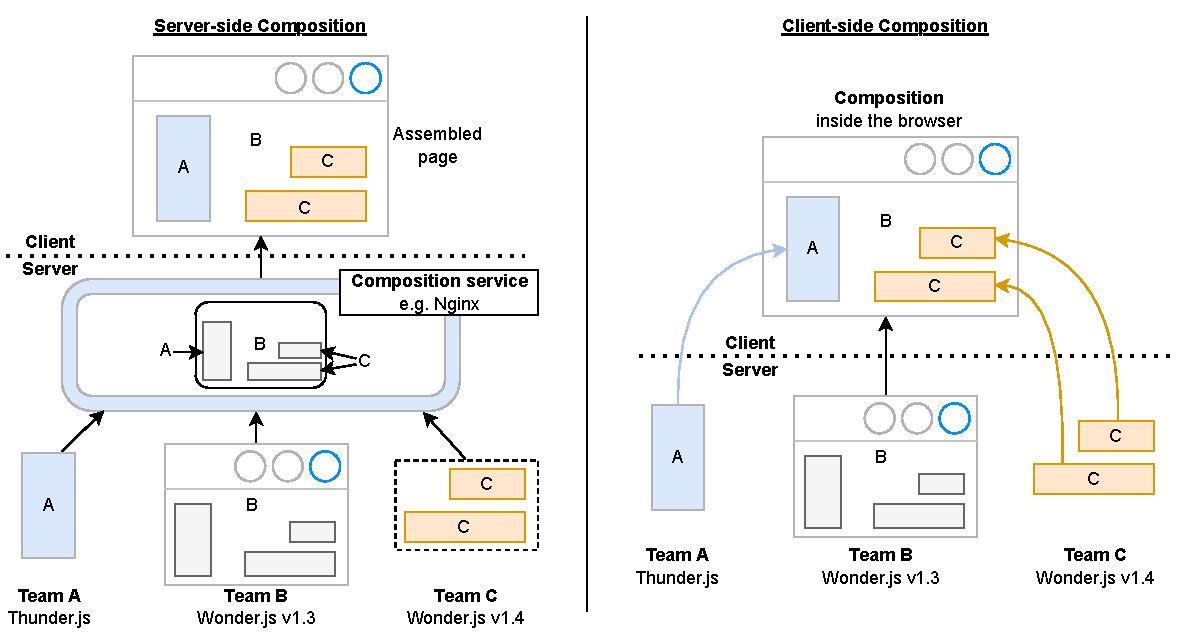
\includegraphics[width=1\textwidth]{img/ServerClientSideComposition}}\\ % Pfad
		\source{\cite[Eigene Darstellung in Anlehnung an][60,86]{Geers2020}} % Quelle
		\label{fig:ServerClientSideComposition}
	\end{minipage}
\end{figure}

Dadurch, dass die gesamte Webseite auf dem Server zusammengesetzt und als vollständige Lösung an den Nutzer ausgegeben wird, sind gute Ladezeiten zu erreichen.\footnote{\cite[vgl.][60]{Geers2020}}

Bei Nginx, einer Softwarelösung für unter anderem Webserver, Cache, Lastverteilung und Reverse Proxy,\footnote{\cite[vgl.][]{nginx2022}} werden die einzelnen Fragmente durch \textit{\gls{SSI}} serverseitig zusammengesetzt. Die Seite, welche später an den Client ausgegeben wird, beinhaltet noch Platzhalter. Diese werden durch \gls{SSI} mit dem Zielinhalt ersetzt. In Anhang \ref{app:Listing} unter \cref{list:SSIPlaceholder} ist ein exemplarischer Platzhalter dargestellt.

Die Platzhalter beinhalten den Pfad zum Code, durch welchen sie ersetzt werden sollen. Alle Platzhalter, die sich auf der auszugebenden Seite befinden, werden anschließend durch den referenzierten Code ersetzt. In der \cref{fig:SSCNginxSSI} in Anhang \ref{app:Bilder} ist ein Sequenzdiagramm dargestellt, welches die einzelnen Schritte im Detail darstellt.

\textit{Server-side Composition} bietet Vorteile durch schnelle Performance, weil der Browser direkt eine fertig zusammengesetzte Webseite geliefert bekommt. Ebenfalls ist \gls{SSI} als Technologie bewährt und \textit{Server-side Composition} ist suchmaschinenfreundlich.\footnote{\cite[vgl.][82\psq]{Geers2020}}

Die Nachteile von \textit{Server-side Composition} kommen vor allem bei großen, dynamischen Anwendungen zu Tage. Es dauert, bis alle Teile der großen Anwendung gerendert und zum Client übertragen werden. Eine Mischung von \textit{Server-} und \textit{Client-side Composition} könnte helfen, die Ladezeit zu verbessern. Ebenfalls wirken Server-side Applikationen nicht sehr interaktiv auf den Anwender. Programmteile die schnell reagieren und auf Nutzereingaben interagieren müssen, sollten für verringerte Ladezeiten clientseitig zusammengesetzt werden.\footnote{\cite[vgl.][83]{Geers2020}}

\textit{Server-side Composition} ist für den weiteren Verlauf der \dokumententyp{}
 nicht von Relevanz und wurde nur für die Gegenüberstellung zu \textit{Client-side Composition} genutzt, welche im nachfolgenden \cref{sec:ClientSideComposition} erklärt wird.

\subsubsection{Client-side Composition}\label{sec:ClientSideComposition}

Bei der \textit{Client-side Composition} werden die Fragmente einzeln heruntergeladen und erst beim Client im Browser zusammengesetzt. Auch dieser Vorgang ist in der vorherigen \cref{fig:ServerClientSideComposition} dargestellt.

Im Gegensatz zu \textit{Server-side Composition} werden bei der \textit{Client-side Composition} die einzelnen Fragmente im Browser des Client generiert und zusammengesetzt. Lösungen dafür sind beispielsweise die gängigen Javascript-Frontend-Frameworks \textit{Angular}, \textit{Vue.js} oder \textit{React}.

Je nach Art der Zusammensetzung können die Fragmente auch auf unterschiedlichen Technologien beruhen. So kann Fragment A auf einer neueren Version des Frameworks beruhen, welches die Fragmente zusammensetzt. Fragment B kann sogar auf einer ganz anderen Technologie beruhen, solange es die benötigten Referenzen und Bibliotheken eigenständig mitbringt.

\textit{Client-side Composition} bietet sich bei interaktiven Anwendungen an, wie beispielsweise einer Web Applikation zum Erstellen der Steuererklärung. Eine statische Anwendung kann besser serverseitig zusammengesetzt und mit einzelnen clientseitigen Komponenten versehen werden, bei denen vorwiegend dynamischer Inhalt angezeigt wird.\newline
Ebenfalls ist es durch Iframes und Web Components möglich, eine starke, technische Isolierung der \gls{UI} zu erzielen.\footnote{\cite[vgl.][97]{Geers2020}} Dadurch können sich Fragmente verschiedener Teams in den Stylings nicht überschreiben, was bei \textit{Server-side Composition} nur durch strikte Konventionen, wie beispielsweise Prefixe für CSS-Klassen und Namespaces, möglich ist.\footnote{\cite[vgl.][83]{Geers2020}}

In den nachfolgenden Abschnitten werden drei Arten der clientseitigen Einbindung eines Microfrontends vorgestellt.

\subsubsection{Iframe}\label{sec:IFrame}

Das \textit{Inline Frame} (nachfolgend Iframe) ist ein \gls{HTML} Element, durch welches andere HTML-Webseiten in die bestehende Webseite eingebunden werden können. Es wird von allen aktuellen Browsern unterstützt.\footnote{\cite[vgl.][]{MDNWebDocs2021a}}
Im nachfolgenden \cref{list:iframe} ist ein beispielhaftes Iframe zu sehen, über welches die Webseite der \gls{FHDW} eingebunden wird.

\begin{figure}[bht]
	\begin{lstlisting}[caption=Exemplarische Einbindung einer Webseite über das Iframe-Element, label=list:iframe]
		<iframe id="iframeId" src="https://fhdw.de/" name="FHDW-Webseite" 
		width="500" height="200" style="border: none"></iframe>
	\end{lstlisting}
	\footnoterule{}
	\footnotesize{\textbf{Quelle:} Eigene Darstellung}
\end{figure}

Dem Iframe Element wird über den \texttt{src}-Parameter die \gls{URL} der einzubindenden Webseite mitgegeben. Über die Parameter \texttt{width} und \texttt{height} können Anpassungen an der Breite und Höhe des Elements, in dem die eingebundene Webseite angezeigt wird, getätigt werden. Dies ist erforderlich, sollte die Standardauflösung von 300px x 150px nicht ausreichen.\footnote{\cite[vgl.][]{MDNWebDocs2021a}}

Ebenfalls kann über den \texttt{style}-Parameter eigener \gls{CSS} Code auf das \gls{HTML}-Element angewendet werden. Durch diesen Parameter kann unter anderem der standardmäßige Rahmen ausgeblendet werden, um die Einbindung einer externen Ressource für den Anwender weniger offensichtlich zu machen.

Ein Iframe kann, wenn es in eine andere Anwendung eingebunden wird, diese nicht durch Styles beeinflussen. Die Kapselung der UI ist dementsprechend hoch gegenüber anderen Microfrontends.

Das Iframe eignet sich als schnelle Art der Einbindung mit hoher Kapselung des Inhalts gegen andere Microfrontends. Iframes haben eine schlechte Performance, wenn viele von ihnen eingebunden werden. Jedes Iframe erstellt einen neuen Browserkontext, welcher Rechen- und Speicherintensiv ist. Ebenfalls sind Iframes für Screenreader und Suchmachinen nicht gut zu erreichen, was in geringer Suchmaschinenoptimierung und geringer Barrierefreiheit resultiert.\footnote{\cite[vgl.][35]{Geers2020}}

\subsubsection{Web Components}\label{sec:Webcomponents}

Web Components bestehen aus drei Technologien: \textit{Shadow DOM}, \textit{Custom Elements} und \textit{HTML Templates}.\footnote{\cite[vgl.][]{MDNWebDocs2022a}}

Durch das \textit{Shadow \gls{DOM}} wird einem \gls{HTML}-Element ein eigener, sogenannter Shadow, \gls{DOM} Tree gehängt. Dieser Tree wird vom Browser separat und unabhängig vom Main \gls{DOM} gerendert. Das separate Rendering der beiden \gls{DOM}s hat zur Folge, dass diese voneinander abgekapselt agieren und sich nicht gegenseitig beeinflussen können. So haben \gls{CSS}-Konfigurationen innerhalb des Shadow \gls{DOM} Trees keine Auswirkungen auf Elemente außerhalb des eigenen Trees. Dadurch wird vermieden, dass eingebundener Code die einbindende Webseite beeinflusst und zugleich nicht von \gls{CSS}-Konfigurationen der einbindenden Webseite beeinflusst wird.

Die Elemente im Shadow \gls{DOM} zu Kapseln hat Vor- und Nachteile. Durch den eigenen \gls{DOM} ist die Isolierung des Codes gegenüber anderen Microfrontends, wie bei Iframes auch, sehr stark. Ebenfalls können globale Styles die Web Component nicht beeinflussen, was bei legacy Anwendungen ein Vorteil ist. 
Auf der anderen Seite wird Shadow \gls{DOM} in alten Browsern nicht unterstützt und die Kapselung der Styles ist mit einigen Design Frameworks nicht kompatibel. Beispiele für inkompatible Frameworks sind Twitter Bootstrap oder Angular Material.\footnote{\cite[vgl.][96]{Geers2020}}

Für wiederverwendbaren \gls{HTML} Code werden \textit{\gls{HTML} Templates} verwendet. Ein Template wird über den \gls{HTML}-Tag \texttt{template} definiert und der Inhalt dessen bleibt beim Laden der Seite erst einmal verborgen. Das Template kann später je nach Bedarf ein oder mehrere Male über \gls{JS} nachgeladen werden. Ein beispielhaftes Template ist in Anhang \ref{app:Listing} in \cref{list:HTMLTemplate} dargestellt.

Durch \textit{Custom Elements} wird ermöglicht, dass neben den vordefinierten \gls{HTML} Tags noch weitere, individuelle \gls{HTML} Tags der Webseite hinzugefügt werden können. Der Inhalt eines Templates kann zu einem \textit{Custom Element} Tag hinzugewiesen werden. Die dahinterliegende \textit{Custom Elements} API rendert aus dem individuellen \gls{HTML} Tag dann anschließend den definierten Inhalt.\footnote{\cite[vgl.][]{Rauber2021}}

Web Components sind ein anerkannter Webstandard, der direkt mit der Browser \gls{API} interagieren kann. Die starke Isolation des Inhaltes bei Bedarf sorgt für eine robuste Einbindung.\footnote{\cite[vgl.][96\psq]{Geers2020}} Dafür benötigen Web Componentens auch \gls{JS} clientseitig und unterstützen kein serverseitiges Rendering. Dies ist zwar über Umwege realisierbar, aber nicht der vorgesehene Standard, was bei Anforderungen an geringe initiale Ladezeiten von Nachteil ist.\footnote{\cite[vgl.][97\psq]{Geers2020}}

\subsubsection{Webpack Module Federation}\label{sec:ModuleFederation}

Webpack ist ein OpenSource Modulbundler, welcher Module und deren Abhängigkeiten in statische Pakete umwandelt. Das Frontend Framework Angular benutzt Webpack zum Transpilieren, Kompilieren und Veröffentlichen von Quellcode.\footnote{\cite[vgl.][133]{Clow2018}}

Mit der Major Version 5 von Webpack, welche im Oktober 2020 offiziell erschienen ist, wurde ein neues Feature namens \textit{Module Federation} vorgestellt.\footnote{\cite[vgl.][]{Webpack2020a}} Durch Module Federation sind zwei neue Plugins hinzugekommen: Das \textit{ContainerPlugin} und das \textit{ContainerReferencePlugin}.

Das \textit{ContainerPlugin} ermöglicht asynchronen Zugriff auf Module, welche in einem Container zur Verfügung gestellt werden. Das \textit{ContainerReferencePlugin} ermöglicht Referenzen zu anderen, entfernten Containern, wodurch Module aus diesen entfernten Containern importiert und genutzt werden können.\footnote{\cite[vgl.][]{Webpack2020b}}

Die Entwickler von Webpack beschreiben zwei Anwendungsfälle. Mit dem Ersten können klassische Microfrontend Applikationen realisiert werden. So sind alle Unterseiten einer Webseite als eigene Container veröffentlicht, welche ihren Inhalt als Modul bereitstellen. Die zentrale Seite, beispielsweise die Startseite der Webseite mit Navigationseinträgen im Header- und Seitenbereich, referenziert als Application Shell durch das \textit{ContainerReferencePlugin} alle Unterseiten und bindet deren Content ein. Des Weiteren stellt die Application Shell gängige Bibliotheken bereit, auf die die Unterseiten zugreifen können. Da die Bibliotheken geteilt werden ist sichergestellt, dass diese nur einmal geladen werden.\footnote{\cite[vgl.][]{Webpack2020b}}

Das unabhängige Einbinden der Seiten hat zur Folge, dass die Unterseiten alle einzeln neu veröffentlicht werden können, wenn neuer Inhalt für eine neue Version bereit steht. Die aufrufende Seite muss nur dann neu veröffentlicht werden, wenn Änderungen an den Links vorgenommen werden. Wird lediglich der Inhalt der Unterseiten geändert, ist keine neue Veröffentlichung der Hauptseite erforderlich.\footnote{\cite[vgl.][]{Webpack2020b}}

Beim zweiten Anwendungsfall wird eine Komponentenbibliothek, bspw. ein \gls{SDK}, zum Einbinden zur Verfügung gestellt. Alle Apps, die mit diesem \gls{SDK} arbeiten, integrieren es mittels Module Federation in ihre Applikation. Wenn eine neue Version des \gls{SDK}s veröffentlicht werden soll, muss nur das Modul des \textit{ContainerPlugins} neu veröffentlicht werden und nicht jede einbindende App.\footnote{\cite[vgl.][]{Webpack2020b}}

\textbf{Module Federation in Angular}\\
Webpack ist der Modulbundler für Angular. Seit Angular Version 11 wird Webpack in der Major Version 5 unterstützt. Dadurch ist mit Module Federation ein weiterer Weg zur Einbindung eines Microfrontends in eine Portalshell hinzugekommen. Module Federation ermöglicht es, Programmteile zu referenzieren die zur Compilezeit noch nicht bekannt sind. Ebenfalls können sich verschiedene Microfrontends Bibliotheken teilen, sodass diese nur einmal vom Client geladen werden müssen.\footnote{\cite[vgl.][39]{Steyer2020}}

Damit eine Applikation mittels Module Federation eingebunden werden kann, müssen auf beiden Seiten Konfigurationen vorgenommen werden. In der nachfolgenden \cref{fig:ModuleFederation} sind die notwendigen vier Schritte zur Einbindung dargestellt.

\begin{figure}[hbt!]
	\centering
	\begin{minipage}[t]{0.64\textwidth}	
		\caption{Notwendige Konfigurationen für Module Federation}
		\frame{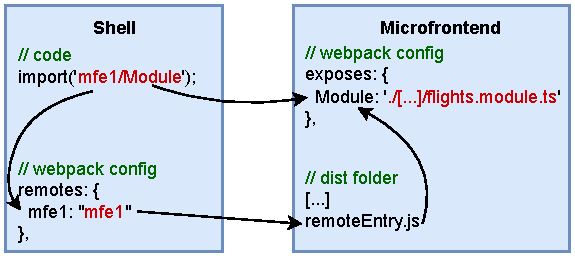
\includegraphics[width=1\textwidth]{img/ModuleFederationConfig.pdf}}\\ % Pfad
		\source{\cite[Eigene Darstellung in Anlehnung an][]{Steyer2020a}} % Quelle
		\label{fig:ModuleFederation}
	\end{minipage}
\end{figure}

Jede Applikation, die Module Federation einsetzt, muss über eine \texttt{webpack.config.js}-Datei verfügen. Über diese Datei wird Webpack konfiguriert und die Module der Applikation aufgelistet, welche exportiert und importiert werden sollen. Die Portalshell referenziert ein entferntes Modul. Dieses Modul wird von einem Microfrontend exportiert und in die \texttt{remoteEntry.js}-Datei im \textit{dist}-Ordner von Webpack geladen. Der Pfad zu diesem Ordner ist in der Konfiguration der Shell hinterlegt.

In \cref{lst:ModuleFederationWebpackRemote} in Anhang \ref{app:Listing} ist der relevante Teil einer \texttt{webpack.config.js}-Datei für eine RemoteApp zu sehen. Die RemoteApp veröffentlicht in der \texttt{remoteEntry.js}-Datei das Angular Distant-Modul mit dem Namen \textit{microapp}.

In \cref{lst:ModuleFederationWebpackShell} in Anhang \ref{app:Listing} ist der dazugehörige relevante Teil einer \texttt{webpack.config.js}-Datei einer Shell zu sehen. 
Die Shell bindet das RemoteModul \textit{microapp} ein, welches unter \texttt{microapp@http://localhost:3000/remoteEntry.js} zu finden ist. Das @-Zeichen trennt dabei den Namen des Microfrontends von der \gls{URL} des Microfrontends.

Ebenfalls sind in der Konfiguration der Shell die Bibliotheken zu sehen, welche für die RemoteApps zur Verfügung gestellt werden. Im Beispiel von \cref{lst:ModuleFederationWebpackShell} in Anhang \ref{app:Listing} werden die vier gängigen Angular Bibliotheken \textit{@angular/core}, \textit{@angular/common}, \textit{@angular/common/http} und \textit{@angular/router} zur Verfügung gestellt. Das Microfrontend hat die gleichen Bibliotheken als geteilt konfiguriert und greift auf die Bibliotheken der Shell zurück, anstatt sie selbst mitzubringen.

Damit die Shell mit dem Microfrontend Daten austauschen kann, muss in den Konfigurationsdateien beider Seiten ein \texttt{SharedMapping}-Objekt referenziert werden. 
Dort kann eine individuelle Angular Library\footnote{\cite[Für weitere Informationen siehe][]{Angular2022h}} eingebunden werden, welche von der Shell befüllt und vom Microfrontend konsumiert wird.\footnote{\cite[vgl.][]{Steyer2021d}}

\textbf{Module Federation mit Web Components}\\
Mit Module Federation ist es ebenfalls möglich, neben Angular Modulen und Komponenten, auch Web Components zu Teilen. Dies ist dann sinnvoll, wenn die einbindende Shell über eine andere Framework Version als das Microfrontend verfügt.

Dafür muss das Microfrontend in der \texttt{app.module.ts} die zu exportierende Angular Komponente als \texttt{customElement} definieren, analog wie in \cref{sec:Webcomponents} beschrieben. In der Webpack Konfiguration muss anstelle des Modules die \texttt{bootstrap.ts} veröffentlicht werden.
Statt eines Modules wie bei der vorherigen Variante, lädt die Portalshell ein Script von dem RemoteEntry.\footnote{\cite[vgl.][]{Steyer2021a}}

Durch das Einbinden einer Web Component können Microfrontends einer anderen Angular Major Version geladen und geteilt werden. Ebenfalls können Web Components eingebunden werden, die in einem anderen Web Frontend Framework erstellt wurden (bspw. in React). In  \cref{fig:ModuleFederationSchnittmengenFrameworks} in Anhang \ref{app:Bilder} sind Schnittmengen von vier Microfrontends mit einer Shell skizziert. Bibliotheken mit gleicher Major Versionsnummern können geteilt werden, wie es bei \gls{MFE2} und \gls{MFE3} der Fall ist. Module Federation wählt automatisch die Bibliothek mit der höheren Minor Version und teilt sie zwischen Shell und Microfrontend. Microfrontends mit anderen Web Frameworks, wie das React \gls{MFE4} in der Abbildung, müssen vollständig zum Client übertragen werden.
 
\subsubsection{Auswirkungen der Entscheidungsvielfalt}\label{sec:Entscheidungsvielfalt}

In diesem abschließenden Abschnitt sollen die Auswirkungen der großen Entscheidungsvielfalt beim Thema Microfrontends verdeutlicht werden. In den vorherigen Abschnitten wurde auf die Architektur von Microfrontends, Portalapplikationen und verschiedene Microfrontend-Varianten eingegangen. Je nachdem, welche Entscheidungen Softwarearchitekten für die Applikationen treffen, ergeben sich unterschiedliche Konsequenzen für die verwendeten Technologien.

Die Softwarearchitekten, welche eine Microfrontend-Architektur auswählen, müssen verschiedene Entscheidungen treffen. Diverse Lösungsarten für Komposition und Routing sind in der nachfolgenden \cref{fig:TrennungRoutingStrategien} dargestellt.

\newpage
\begin{figure}[hbt!]
	\centering
	\begin{minipage}[t]{0.8\textwidth}	
		\caption{Weiterleitung und Zusammensetzung von Microfrontends}
		\frame{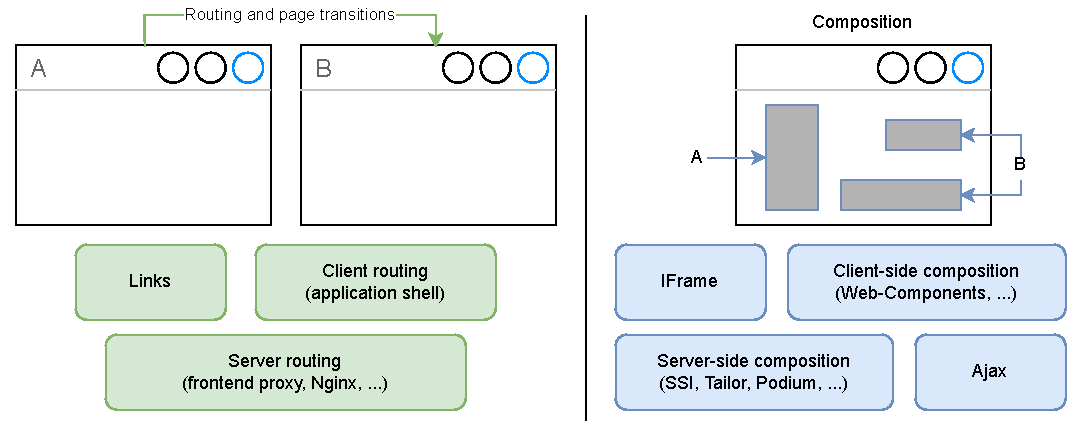
\includegraphics[width=1\textwidth]{img/TrennungRoutingStrategien}}\\ % Pfad
		\source{\cite[Eigene Darstellung in Anlehnung an][5]{Geers2020}} % Quelle
		\label{fig:TrennungRoutingStrategien}
	\end{minipage}
\end{figure}

Wenn durch das Routing die Seite wechselt oder sichtbar neu geladen werden muss, wird nachfolgend von \textit{hartem Routing} gesprochen. Das Gegenstück dazu ist \textit{softes Routing}, bei welchem die Seiteninhalte dynamisch ohne Übergang ausgetauscht werden. Das Routing bestimmt das Benutzererlebnis und kann mit hartem Routing durch Links realisiert werden, oder aber auch client- oder serverseitig geschehen. Bei den gängigen Web Fontend Frameworks sind Lösungen für softes Routing enthalten, wie beispielsweise der \textit{Angular Router} bei Angular. Softes Routing ist für den Benutzerkomfort zu empfehlen, wohingegen ein hartes Routing durch Links den Wechsel in eine andere Webseite der Produktpalette eines Unternehmens signalisiert.

Das Einbinden der Microfrontends in eine Shell kann durch verschiedene Techniken realisiert werden. Alle haben Vor- und Nachteile. Es muss anhand des gegebenen Anwendungsfalles jeweils individuell entschieden werden, welche dieser Techniken zum Einsatz kommen.

Ein möglicher Entscheidungsbaum ist nachfolgend in der \cref{fig:EntscheidungsbaumArchitektur} dargestellt. Die Abbildung bietet anhand der Anforderungen eine Entscheidungshilfe bei der Auswahl der Kompositionstechnik des Frontends.

\newpage
\begin{figure}[hbt!]
	\centering
	\begin{minipage}[t]{0.8\textwidth}	
		\caption{Microfrontend-Architektur Entscheidungsbaum nach Geers}
		\frame{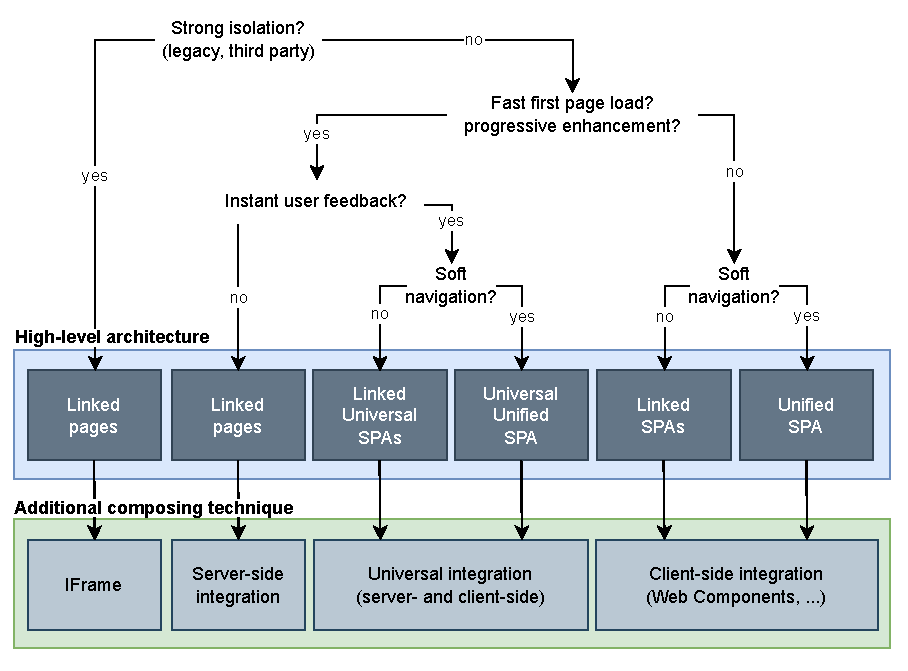
\includegraphics[width=1\textwidth]{img/EntscheidungsbaumArchitektur}}\\ % Pfad
		\source{\cite[Eigene Darstellung in Anlehnung an][166]{Geers2020}} % Quelle
		\label{fig:EntscheidungsbaumArchitektur}
	\end{minipage}
\end{figure}

Die Entscheidung zur Art der Einbindung hängt davon ab, welche Isolation gewünscht ist, wie sich die App beim Navigieren verhalten soll und ob Wert auf initiale Ladezeiten gelegt wird.

Andere Autoren haben ähnliche Entscheidungsbäume veröffentlicht. So hat beispielsweise Manfred Steyer 2018 einen Leitfaden zu Microfrontends anhängig von Architekturzielen veröffentlicht (siehe \cref{fig:EntscheidungsbaumArchitekturMF} in Anhang \ref{app:Bilder}), welcher allerdings Module Federation noch nicht beinhaltet.\footnote{\cite[vgl.][]{Steyer2018}}